\documentclass[11pt]{article}
\usepackage[margin=1in]{geometry}
\usepackage{amsmath}
\usepackage{amssymb}
\usepackage{amsthm}
\usepackage{graphicx}
\usepackage{booktabs}
\usepackage{multirow}
\usepackage{array}
\usepackage{threeparttable}
\usepackage{setspace}
\usepackage[round]{natbib}
\usepackage[hidelinks]{hyperref}
\usepackage{caption}
\usepackage{enumitem}
\usepackage{tikz}
\usetikzlibrary{positioning}
\usepackage{pgfplots}
\pgfplotsset{compat=1.17}
% Figures are drawn natively in pgfplots (no external files needed).
% make_figures_v2.py remains as an optional matplotlib alternative.
\definecolor{npblue}{RGB}{31,78,121}
\definecolor{npmid}{RGB}{72,120,168}
\definecolor{gred}{RGB}{176,74,74}
\definecolor{gold}{RGB}{200,162,74}
\captionsetup{font=small,labelfont=bf}
\setstretch{1.15}
\emergencystretch=1.5em
% float discipline: let tall tables place instead of queueing to the end
\renewcommand{\topfraction}{0.92}
\renewcommand{\bottomfraction}{0.6}
\renewcommand{\textfraction}{0.06}
\renewcommand{\floatpagefraction}{0.8}
\graphicspath{{figures/}}

\newcommand{\PP}{\mathbb{P}}
\newcommand{\VaR}{\mathrm{VaR}}
\newcommand{\ES}{\mathrm{ES}}
\newtheorem{proposition}{Proposition}
\newtheorem{lemma}{Lemma}
\newtheorem{corollary}{Corollary}
\theoremstyle{remark}
\newtheorem{remark}{Remark}

\title{When Do Flexible Tail-Risk Models Beat GARCH?\\
\large Post-Shock Scale Error, Residual Shape, and a Real-Time Score}
\author{%
  Sean Qin\thanks{E-mail: \texttt{sean.qin@u.northwestern.edu}.}\\[4pt]
  \normalsize Department of Statistics and Data Science, Northwestern
  University, Evanston, IL 60208}
\date{November 2026}

\begin{document}
\maketitle

\begin{abstract}
Flexible tail-risk models beat GARCH(1,1)-$t$ on about one asset-day in ten, and a trailing kurtosis of the filter's own residuals identifies those days in advance. On 200 US stocks a pooled gradient-boosted residual model and SAV-CAViaR gain about 3\% of pinball loss in the score's top decile, more after positive shocks than negative ones, and little elsewhere. A top-decile score records one recent shock of about eight conditional standard deviations, after which GARCH overstates variance. A Beta-$t$-EGARCH, which bounds that response, beats both flexible models there. A smaller residual-shape gain survives on the robust scale.
\end{abstract}

\noindent\textbf{Keywords:} Value-at-Risk; Expected Shortfall;
forecast evaluation; robust volatility; quantile regression; misspecification.

\medskip
\noindent\textbf{JEL classification:} C14; C52; C53; C58; G17.

%% ===== INTRODUCTION =====
\section*{Introduction}\label{sec:intro}

Flexible tail-risk models, from filtered historical simulation and CAViaR to gradient-boosted and neural quantile learners, are regularly reported to forecast Value-at-Risk (VaR) and Expected Shortfall (ES) better than GARCH-type benchmarks \citep{kuester2006, nietoruiz2016, chronopoulos2024}. An average gain says little about where it is earned. This paper asks two questions of it on a panel of 200 US stocks, scored on 221.6k test asset-days (one name on one trading date) with inference over dates: on which asset-days does a flexible model beat GARCH(1,1)-$t$, and why does it beat it there?

The answer to the first question is narrow. The advantage sits on about one asset-day in ten, and those days can be flagged the day before from the filter's own output, the trailing 63-day excess kurtosis of its standardized residuals, the oldest specification diagnostic for a GARCH filter \citep{bollerslev1987, hansen1994ARCD}, used as a rank. In the top decile of that score a pooled gradient-boosted model of the residual quantile improves on GARCH-$t$ by $+2.98\%$ of pinball loss (per-date Diebold--Mariano statistic, DM, 10.5), the ninth decile carries a smaller edge ($+0.46\%$, DM 2.9), and the other eight are within noise. SAV-CAViaR \citep{engle2004caviar}, which models the return quantile directly and shares nothing with the learner, has the same profile ($+2.81\%$, DM 8.2, in the top decile; $+0.08\%$, DM 1.6, below it). The conditional predictive ability test of \citet{giacominiwhite2006} rejects equal accuracy given the lagged score. The concentration replicates on an untouched 2000--2013 holdout under a specification frozen in advance, in a point-in-time universe that keeps delisted names, under strict calendar splits, and under annual refits, where the average edge is within noise and the top-decile edge is not.

The answer to the second question starts from what a top-decile score records. In all but a handful of top-decile windows a single residual carries more than half of the window's centered fourth-moment sum (median 97\%). Its median size is 8.2 conditional standard deviations, it can fall anywhere in the three-month window (median 31 trading days before the forecast), and removing it returns the window's kurtosis to the level of the fifth decile. A high score is a record of one large shock in the recent past. After such a shock a GARCH(1,1) raises its conditional variance in proportion to the squared shock and keeps it high for weeks, the outlier sensitivity documented by \citet{carnero2007outliers} and addressed by \citet{muler2008robust} and \citet{boudt2013robust}, so the residuals that follow are too small for the Student-$t$ tail the filter is paired with. A flexible residual model given the filter's scale state learns to pull its tail in. The sign of the shock matters in the way the jump literature predicts: in individual stocks a negative jump raises subsequent volatility and a positive one lowers it \citep{pattonsheppard2015}, and the flexible model's top-decile edge is $+3.9\%$ after a positive shock (DM 7.1) and $+1.6\%$ after a negative one (DM 5.4).

Bounding the shock's influence on the variance measures how much of the advantage that is. A GARCH whose news term is capped at three conditional standard deviations, with the Student-$t$ tail unchanged, beats standard GARCH-$t$ by $+3.17\%$ (DM 8.2) in the top decile, more than the flexible model's $+2.98\%$, and against the capped filter the flexible model's top-decile edge falls to $+0.45\%$ (DM 4.7). A Beta-$t$-EGARCH \citep{harvey2013dynamic}, fitted by maximum likelihood and robust to a single shock by construction, beats GARCH-$t$ by $+3.56\%$ (DM 8.8) in the top decile, and it beats both flexible models there: the pooled gradient-boosted model by $0.64\%$ (DM 2.6) and SAV-CAViaR by $0.78\%$ (DM 3.7). On large caps with intraday data a realized-variance scale leaves the score's edge within noise. For both flexible models, most of the gain over GARCH-$t$ is a scale correction that a robust filter delivers on its own, and some of the gains over GARCH(1,1) reported for flexible tail models may be the same correction.

A smaller part of the gain is shape. Rebuilt on the Beta-$t$-EGARCH scale, the flexible residual model beats that model's own Student-$t$ tail by $+0.27\%$ (DM 2.0) in the top decile and is within noise elsewhere, and it lowers the joint $(\VaR,\ES)$ loss, the zero-homogeneous Fissler--Ziegel (FZ0) score of \citet{fissler2016} and \citet{patton2019}, at both regulatory levels, under frozen fits (DM 3.9 at 1\%, 4.7 at 2.5\%) and under annual refits (DM 3.1 and 2.7). The residual-shape component is real, small, and located in the tail.

The estimator behind these comparisons follows the two-step logic of filtered historical simulation and GARCH-EVT \citep{baroneadesi1999fhs, mcneilfrey2000}: a GARCH-$t$ scale times a residual quantile from gradient-boosted trees, pooled across names and conditioned on recent residual state, with a pooled extreme-value lower tail. It is the instrument of the paper, not its claim. On FZ0 it beats GARCH-$t$, every FHS variant, GARCH-EVT, EWMA, historical simulation, and the score-driven GAS model of \citet{patton2019}; it ties GJR-GARCH-skew-$t$ at both regulatory levels and the ES-CAViaR of \citet{taylor2019} at 2.5\%; and Beta-$t$-EGARCH scores lower than it at both levels under frozen fits (significantly at 2.5\%, DM 2.5) and is within noise of it under annual refits. Table~\ref{tab:configs} lists each configuration the paper reports, the claims it carries, and the rules fixed before the test data were scored.

The practical reading is a monitor. The score marks the days on which a GARCH(1,1)-$t$ in production is stressed, mostly through its own post-shock scale and partly through its shape. On the panel, a rule that runs Beta-$t$-EGARCH on those days and GARCH-$t$ otherwise is significantly better than GARCH-$t$ on FZ0 at both levels and statistically equal to running the robust filter everywhere. The rule was designed on those rows, and on thirty-two instruments outside the panel it does not beat GARCH-$t$ (Online Appendix), so it describes where the gain sits and is not offered as a tested rule. The edges are reductions in consistent scoring functions \citep{gneiting2011}, percentage reductions in average loss, not monetary measures, and the paper makes no capital claim.

The contribution is empirical and diagnostic. Where flexible tail models beat GARCH, measured with date-level inference and familywise control, is a narrow set of states identifiable in advance, and why they beat it there is, for both flexible models studied, mostly a correction to the filter's scale. Its ingredients are known: GARCH overreacts to outliers \citep{carnero2007outliers}, jumps are less persistent than continuous variation \citep{andersen2007roughing}, and a score-driven filter forecasts a single index better than $t$-GARCH on the day after an extreme return \citep{blazsek2018extreme}. The comparison literature, meanwhile, ranks flexible and parametric models by average loss and backtests over a sample \citep{kuester2006, nietoruiz2016}. What we add is the measurement that the post-shock scale error accounts for most of the flexible models' advantage over GARCH, across a panel, on days a score flags in advance. The evidence is for individual US stocks. On fourteen stocks outside the training pool the robust filter's post-shock advantage replicates, and on eighteen instruments in other asset classes it does not appear (Section~\ref{sec:frontier}).

\medskip\noindent The paper proceeds as follows.
Section~\ref{sec:background} places the question in the forecasting literature and defines the benchmarks. Section~\ref{sec:methods} sets out the estimator and the score, and Section~\ref{sec:protocol} the data and the evaluation protocol. Section~\ref{sec:frontier} locates the advantage and decomposes it into scale and shape. Section~\ref{sec:frtb} reports the joint VaR and ES evaluation. Section~\ref{sec:applications} covers the use of the score, and Section~\ref{sec:limitations} concludes.

\section{Related literature and benchmark models}\label{sec:background}

\subsection{Risk measures and the FRTB discipline}

For a return $r_{t+1}$ with conditional law $F_t$, the level-$\alpha$
return-space quantile is $q_t^\alpha = F_t^{-1}(\alpha)$ (negative in
the left tail). The return-space Expected Shortfall is
$e_t^\alpha = \mathbb{E}[r_{t+1} \mid r_{t+1} \le q_t^\alpha]$ for continuous
$F_t$. In general $e_t^\alpha=\alpha^{-1}\!\int_0^\alpha F_t^{-1}(v)\,dv$, the
coherent form used throughout \citep{artzner1999, acerbitasche2002}.
The regulatory VaR and ES are their negatives (the sign convention is
fixed once in Section~\ref{sec:notation}). FRTB \citep{bcbs2019frtb} sets the capital metric at a stressed $\ES_{97.5}$ over a liquidity-adjusted horizon (ten days for the base bucket), while backtesting remains VaR-exception based. More than twelve exceptions at 99\%, or thirty at 97.5\%, in a 250-day year pushes a trading desk off the internal-models approach. The empirical bar for ``beating the industry standard'' is therefore joint. It requires accuracy on the joint $(\VaR,\ES)$ score at 97.5\% \citep{fissler2016, patton2019}, since ES alone cannot be scored \citep{gneiting2011}, and on pinball, together with the unconditional-coverage test of \citet{kupiec1995} and the conditional-coverage test of \citet{christoffersen1998}, the joint likelihood-ratio test of correct coverage and breach independence, at both levels. Significance is assessed by per-date Diebold--Mariano tests \citep{dieboldmariano1995} and the Model Confidence Set \citep{hansen2011mcs}. Real-time monitoring of VaR and ES forecast adequacy is developed by \citet{hoga2023monitoring}; the score of Section~\ref{sec:score} is a cross-sectional, per-asset monitor of the same forecasts, used to rank states rather than to signal a structural break.

\subsection{The parametric family, the simulation family, and CAViaR}

The comparison set spans the models banks run. It includes historical simulation, exponentially weighted moving average (EWMA) variance with the RiskMetrics decay $0.94$ \citep{riskmetrics1996}, GARCH(1,1)-$t$ \citep{bollerslev1986, bollerslev1987}, and the GJR (Glosten--Jagannathan--Runkle) GARCH-skew-$t$ \citep{glosten1993, hansen1994ARCD}, which adds a leverage term and a skewed innovation density. It also includes GARCH-FHS \citep{baroneadesi1999fhs, hullwhite1998}, which pairs a parametric scale with empirical standardized residuals and is the filtered method that the comparison literature ranks closest to the top \citep{kuester2006, nietoruiz2016}. The strongest non-nested semiparametric rival in the set is SAV-CAViaR (conditional autoregressive value-at-risk) \citep{engle2004caviar}, to which the comparison literature is less favorable at the 1\% level \citep{kuester2006}.
The SAV (symmetric absolute value) specification models the quantile
directly by regression quantiles \citep{koenker1978},
$q_t(\tau) = b_0 + b_1\, q_{t-1}(\tau) + b_2\,|r_{t-1}|$ for a quantile level $\tau$ (defined in Section~\ref{sec:notation}), the
quantile analogue of an absolute-value GARCH recursion (the indirect-GARCH CAViaR is the analogue of the squared recursion).
Standalone GARCH-EVT \citep{mcneilfrey2000}, which \citet{kuester2006} rank first among classical methods, is outside the comparison set of Table~\ref{tab:frtb} because the estimator's EVT stage absorbs its filter-then-tail logic; it is compared on the same rows in Sections~\ref{sec:frontier} and~\ref{sec:frtb}.
A single large return also distorts the GARCH filter itself, because it enters the variance recursion squared, keeps the conditional variance high for weeks, and biases the VaR and ES built on it. \citet{carnero2007outliers} document the effect on GARCH identification and estimation, \citet{muler2008robust} and \citet{boudt2013robust} propose robust estimators and filters, and \citet{grane2014outliers} compare corrections by their effect on risk measures. \citet{mancinitrojani2011} build robust semiparametric VaR predictions for GARCH-type models, and score-driven filters bound a single shock's influence by construction \citep{harvey2013dynamic}. On a single index, \citet{blazsek2018extreme} find that a Beta-$t$-EGARCH forecasts better than a $t$-GARCH on the trading day after an extreme return, the post-shock advantage this paper measures across a panel. In realized-volatility models jumps are less persistent than continuous variation, so separating them improves forecasts most after a jump \citep{andersen2007roughing, corsi2010threshold}. In individual stocks jumps mostly accompany firm-specific news such as earnings \citep{leemykland2008, lee2012jumps}, a negative jump raises subsequent volatility while a positive one lowers it \citep{pattonsheppard2015}, and additive outliers left in the data bias GARCH volatility forecasts \citep{fransesghijsels1999}. Section~\ref{sec:frontier} uses a bounded-news filter of this kind to measure how much of the flexible model's advantage is post-outlier scale error.

\subsection{Distribution-free conditional quantiles and GBC}

For the pooled, cross-sectional design the closest antecedent is
\citet{zhang2024commonality}, who forecast realized volatility with
machine-learning models pooled across stocks and document transfer to previously unseen names. That transfer is evidence of a shared volatility mechanism, which our amortized design also exploits. For the VaR comparison the antecedent is \citet{kuester2006}, and for machine-learning volatility forecasting \citet{bucci2020} and \citet{christensen2023ml}. Deep neural-network quantile regression applied directly to VaR is the recent comparison closest to our nonparametric stage \citep{chronopoulos2024}, and \citet{ormaniec2022lstm} find that an LSTM VaR model's advantage over GARCH comes from reacting faster to changes in volatility. Two further semiparametric VaR and ES papers in this journal are direct precedents: \citet{jiang2022singleindex} estimate a single-index expectile model, and \citet{luo2025midas} select low-frequency predictors for joint tail forecasts through a GARCH-MIDAS design with adaptive-Lasso selection. Our object differs from both. We propose no new volatility model and select no predictors; we ask when an observable signal identifies the states in which flexible tail forecasts beat parametric ones, and we decompose the source of that conditional advantage. Relative to the pooled-volatility literature, our object is state dependence in conditional tail-risk forecast performance rather than average realized-variance forecast performance, with the regulatory tail held to calibration, exception-test, and capital discipline. The question here
is where a flexible model helps at all: on roughly ninety percent of
asset-days it does not improve on the parametric benchmark, which cautions
against extrapolating average machine-learning superiority to the tails.
Our amortization is also tested on new listings, against own-history benchmarks and against a pooled peer proxy (Section~\ref{sec:applications}). On tabular state, gradient-boosted trees outperform the implicit quantile network, the reverse of the intraday ranking in \citet{zhang2024commonality}, where neural networks dominate tree-based models. At their daily horizon that dominance already disappears, and our target is a residual quantile curve rather than realized variance, with a different feature set.

The nonparametric family estimates $Q_\phi(\tau \mid s_t)$ directly by pinball-loss empirical risk minimization \citep{koenker1978, steinwart2011}: gradient-boosted quantile trees \citep{friedman2001}, used throughout, and the implicit quantile network of \citet{dabney2018iqn}, the architecture at the core of generative Bayesian computation \citep{polson2023gbc, nareklishvili2025gqbp} in the generalized-Bayes tradition of \citet{jiang2008gibbs} and \citet{bissiri2016general}, retained as a benchmark. Split-conformal prediction \citep{vovk2005, lei2018, romano2019cqr} and its adaptive form \citep{gibbs2021aci} supply the coverage correction of Stage~4, and \citet{barber2023} bound its coverage loss when exchangeability fails.

%% ===== METHODS (notation, estimator, tree/IQN estimator, formal results, toy, Polson delta, misspec score) =====
\section{Semiparametric VaR and ES model}\label{sec:methods}

Each estimator below can be reimplemented from the formulas and
algorithm boxes given. The Online Appendix opens with a glossary of
acronyms and a schematic of the full pipeline, and states the amortized
estimation loop and the monitoring procedure as Algorithms OA.1 and
OA.2.

\subsection{Notation and objects}\label{sec:notation}

Let $r_t$ be the return of an asset on day $t$ and $\mathcal{F}_{t-1}$ the information available before $t$. The conditional $\tau$-quantile of $r_t$ given $\mathcal{F}_{t-1}$ is $Q_t(\tau) = \inf\{q : \Pr(r_t \le q \mid \mathcal{F}_{t-1}) \ge \tau\}$, the number the return falls below with probability $\tau$. Throughout, $\tau\in(0,1)$ is a generic quantile level and $\alpha\in\{0.01,0.025\}$ denotes the reported regulatory levels; both index the same object. One sign convention is used throughout. The paper works in \emph{return space}, with $q_\tau = Q_t(\tau) < 0$ in the left tail and $e_\tau = \tau^{-1}\int_0^{\tau} Q_t(v)\,dv \le q_\tau$, the coherent form of Expected Shortfall \citep{artzner1999, acerbitasche2002}. This is the convention of the FZ0 scoring function ($v,e<0$) \citep{fissler2016, patton2019} and of each table, where ES values such as $-6.37$ are return-space conditional means. The regulatory \emph{loss-space} numbers are their negatives, $\VaR^{\mathrm{loss}}_\tau=-q_\tau$ and $\ES^{\mathrm{loss}}_\tau=-e_\tau$, used only when quoting FRTB levels. The two are never mixed in one expression.

The \emph{standardized residual} $z_t = (r_t-\mu_t)/\sigma_t$ is the return with the model's conditional mean and scale divided out. If the parametric model is right, the $z_t$ are i.i.d.\ draws from one fixed law. The state vector $s_t$ collects trailing realized volatility, the misspecification scores of Section~\ref{sec:score}, and lags, and is what the nonparametric quantiles condition on. A quantile level $\tau \sim \lambda$ is drawn from a base distribution $\lambda$. The shape learners of Section~\ref{sec:gbcmethod} estimate the map from (state, level) to the residual quantile, written $q_\phi(\tau\mid s)$, or $H_\phi(s,\tau)$ for the network.

\noindent\emph{Loss and metric.} All quantile models are trained and
scored by the pinball (check) loss
\begin{equation}
\rho_\tau(x) \;=\; x\,(\tau - \mathbb{I}\{x<0\}),
\qquad x = z - q,
\label{eq:pinball}
\end{equation}
whose expectation is minimized by a conditional $\tau$-quantile
\citep{koenker1978, gneiting2011}---uniquely when that quantile is unique---the way squared
error elicits the mean. Averaging \eqref{eq:pinball} over $\tau\in(0,1)$
targets the whole distribution at once (the integrated loss is the
continuous ranked probability score up to a factor of two, as recorded
below). The loss is density-free, so each estimator below dispenses with a likelihood.

\emph{Choice of scoring function.} Pinball at fixed levels, rather than the continuous ranked probability score that integrates it over all levels \citep{gneitingranjan2011}, keeps the comparison where downside risk lives: the models differ almost entirely in the tail, and a uniform weighting over levels would average those differences away. ES alone is not elicitable \citep{gneiting2011}, so $(\VaR,\ES)$ pairs are scored by the FZ0 loss of Section~\ref{sec:frtb}. Each benchmark is estimated by its own conventional criterion and all are scored out of sample by the same losses (Online Appendix).

\subsection{The final model: the residual-hybrid estimator}\label{sec:hybrid}



The estimator is a four-stage composition in the two-step tradition of filtered historical simulation and GARCH-EVT \citep{baroneadesi1999fhs, hullwhite1998, mcneilfrey2000}. The parametric
filter estimates conditional scale, which it does well and with few
parameters \citep{andersenbollerslev1998, hansenlunde2005}, and the nonparametric stage estimates the state-dependent
shape of the innovation law, which the fixed-shape GARCH-$t$ benchmark fixes by
assumption. The parametric route to a state-dependent shape is the autoregressive conditional density model of \citet{hansen1994ARCD}, and Stage 2 is its distribution-free counterpart. The extreme-value tail extrapolates beyond the estimation
range using the generalized Pareto approximation of Stage~3 below. The
conformal stage corrects the level of the quantile curve using its
realized miss rate, updated daily, the online form of the split-conformal
construction whose exchangeability-based guarantee is Proposition~\ref{prop:conformal}.

\noindent\emph{Motivation for the design.} Conditional scale is identified by a few parameters and estimated with low variance by a parametric filter, so the shape stage is where flexible methods can add value. Per-asset tail data is scarce, which motivates pooling the standardized residuals across names. The EVT stage extrapolates the
tail by the generalized Pareto family \citep{balkema1974,
pickands1975}, and the conformal stage is motivated by the
split-conformal guarantee of Proposition~\ref{prop:conformal}, exact
under exchangeability and approximate for the time-ordered residuals
used here, with a coverage gap bounded by the average total-variation distance between the residual vector and its swapped versions \citep{barber2023}. Whether the four stages together improve on the benchmark out of sample is the question of Sections~\ref{sec:frontier} and~\ref{sec:frtb}.

\emph{Stage 1 (parametric scale).} Fit GARCH-$t$ \citep{bollerslev1986, bollerslev1987},
\begin{equation}
r_t = \mu + \sigma_t z_t,\qquad
\sigma_t^2 = \omega_G + \alpha_G (r_{t-1}-\mu)^2 + \beta_G \sigma_{t-1}^2,
\qquad z_t \sim t_\nu \ \text{(standardized)},
\label{eq:garch}
\end{equation}
by Student-$t$ quasi-maximum likelihood on the estimation window of Section~\ref{sec:protocol} (annually refit in ongoing use), and keep
$\widehat{\mu}$, $\widehat{\sigma}_t$, and the residuals
$\widehat{z}_t = (r_t-\widehat{\mu})/\widehat{\sigma}_t$. The $t_\nu$ likelihood is used to estimate conditional scale; Stages 2 and 3 re-estimate the residual shape. This two-step design, a parametric filter followed by a residual quantile, is the one whose asymptotics \citet{francqzakoian2015} derive for an empirical residual quantile, and \citet{mcneilfrey2000} fit the same filter by Gaussian pseudo-likelihood while explicitly declining to believe the innovation law it assumes. No comparable result covers a pooled tree learner in the second stage, so the paper's inference is on the forecasts (Section~\ref{sec:conventions}).

\emph{Stage 2 (nonparametric shape).} Replace the fixed $t_\nu$
innovation quantile with a state-conditioned quantile model of the
residuals, trained by pinball ERM \emph{pooled across names},
\begin{equation}
\widehat{\phi} \;=\; \arg\min_{\phi}\;
\sum_{\text{names } j}\sum_{\text{days } t}
\mathbb{E}_{\tau\sim\lambda}\,
\rho_\tau\!\big(\widehat{z}_{j,t} - q_\phi(\tau \mid s_{j,t})\big).
\label{eq:shapeERM}
\end{equation}

\emph{Stage 3 (EVT tail).} In the sparsely observed lower tail, where
\eqref{eq:shapeERM} is fitted on few exceedances, use the generalized Pareto
approximation that extreme-value theory motivates for exceedances over
a high threshold, under the standard max-domain-of-attraction
conditions \citep{balkema1974, pickands1975, mcneilfrey2000}. The finite tail mean of the generalized Pareto distribution (GPD) requires $\xi<1$, a condition each fitted tail in this paper
satisfies by a wide margin.\footnote{The peaks-over-threshold formulation uses tail data more efficiently than block maxima \citep{embrechts1997} and is standard in risk management. Here $\xi>0$ is the heavy-tailed case.} On losses $X=-\widehat{z}$, set the threshold $u$ at the empirical $(1-p_0)$ quantile of the pooled training residual losses, with $p_0 = 0.025$. Fit the GPD $G_{\xi,\beta}(y) = 1-(1+\xi y/\beta)^{-1/\xi}$ to the excesses $y = X - u > 0$ by maximum likelihood with location fixed at zero, strictly on past data, giving $(\widehat\xi,\widehat\beta)$; \eqref{eq:evt} is evaluated at these estimates and hats are suppressed below. The shape $\xi$ sets how heavy the tail is and the scale $\beta>0$ how wide; this $\beta$ is the GPD scale, distinct from the GARCH persistence $\beta_G$. One $(\xi,\beta)$ pair is fitted per panel and held fixed across states and levels within a fit. For $\tau \le p_0$, set
\begin{equation}
\widehat{q}^{\,\mathrm{EVT}}(\tau)
\;=\; -\Big[\, u + \tfrac{\beta}{\xi}\big( (\tau/p_0)^{-\xi} - 1 \big)
\Big],
\label{eq:evt}
\end{equation}
which is continuous at its own endpoint, $\widehat q^{\,\mathrm{EVT}}(p_0) = -u$. The formula requires $1+\xi y/\beta>0$, and reduces to $-[u+\beta\log(p_0/\tau)]$ in the $\xi\to0$ exponential limit. The threshold $u$ is unconditional with respect to the state, while the Stage-2 body quantile at $p_0$ is the state-conditional $\widehat q_\phi(p_0\mid s)$, so the two branches need not meet at the join. In the tail the forecast takes the pointwise minimum of the two, the more conservative (more negative) branch, so the pooled GPD extrapolation can tighten a thin state-conditioned body on a stressed day but never loosen it. The curve is then made non-crossing by monotone rearrangement, which cannot move it further from the true quantile curve in any $L^p$ norm \citep{cherno2010rearr}. Both steps are written out in \eqref{eq:hybrid}.

\emph{Stage 4 (conformal finish).} The finished curve is shifted per level by a scalar, $\widetilde{Q}^{z}_t(\tau) = Q^{z}_t(\tau) + c_\tau$ with $Q^{z}_t$ the envelope of \eqref{eq:hybrid}, and the shift is the last operation, after the minimum and the rearrangement. In its static form $c_\tau$ is fixed once: on a held-out calibration split of size $n$, compute the signed errors $\varepsilon_i = \widehat{z}_i - Q^{z}_i(\tau)$ of the envelope and let $c_\tau$ be their $\lceil (n{+}1)\tau \rceil$-th order statistic \citep{vovk2005, lei2018}, the one-sided form of conformalized quantile regression \citep{romano2019cqr}. In the adaptive form used here the shift starts at zero and is updated each day from the panel breach frequency $b_{\tau,t}$ of the shifted forecast, $c_{\tau,t+1} = c_{\tau,t} - \gamma\,(b_{\tau,t}-\tau)$ \citep{gibbs2021aci}, so the shift in force on day $t+1$ uses only breaches observed through day $t$. The \emph{accuracy layer} that carries the FZ0 comparisons of Section~\ref{sec:frtb} and Table~\ref{tab:frtb} sets $c_\tau\equiv0$; the \emph{adaptive overlay} applies the update at both regulatory levels with $\gamma\in\{0.02,0.05\}$, and in era it moves the 97.5\% breach rate toward nominal at no cost in FZ0 (Section~\ref{sec:frtb}). The coverage statement of the static form is standard \citep{vovk2005, lei2018, romano2019cqr} and is restated here for a quantile model $\widehat{q}_\phi$ and its calibration errors.

\begin{proposition}[split-conformal validity under
exchangeability (standard)]\label{prop:conformal}
If the calibration and test errors $\varepsilon_1,\dots,\varepsilon_{n+1}$ are
exchangeable and almost surely distinct (a continuous error
distribution, or randomized tie-breaking), then for each $\tau$ with
$\lceil(n{+}1)\tau\rceil \le n$ the shifted quantile satisfies
\[
\tau \;\le\; \Pr\big(z_{n+1} \le \widehat{q}_\phi(\tau \mid s_{n+1}) + c_\tau\big)
\;=\; \frac{\lceil(n{+}1)\tau\rceil}{n+1}
\;<\; \tau + \tfrac{1}{n+1}.
\]
\end{proposition}
\begin{proof}[Proof sketch]
Under exchangeability and no ties the rank of $\varepsilon_{n+1}$ among
$\{\varepsilon_1,\dots,\varepsilon_{n+1}\}$ is uniform on $\{1,\dots,n+1\}$. The event
$z_{n+1}\le\widehat{q}_\phi(\tau\mid s_{n+1})+c_\tau$ equals $\{\varepsilon_{n+1}\le
\varepsilon_{(\lceil(n+1)\tau\rceil)}\}=\{\mathrm{rank}\le\lceil(n{+}1)\tau\rceil\}$,
whose probability is $\lceil(n{+}1)\tau\rceil/(n+1)\in[\tau,\tau+\tfrac1{n+1})$
\citep{vovk2005}. The full argument is in the Online Appendix, together with the role of the no-ties hypothesis (with ties the upper bound can fail, e.g.\ identical residuals give coverage $1$) and the boundary convention $c_\tau=+\infty$ when $\lceil(n{+}1)\tau\rceil=n+1$. The guarantee is marginal over the state $s_{n+1}$ rather than state-conditional.
\end{proof}

The proposition's scope is narrower than its use. In practice the calibration split necessarily precedes the test period, and time-ordered residuals are not exchangeable, so the proposition only motivates the construction. The static shift fails here for that reason, since the calibration block and the 2020--2024 test era miss on opposite sides of nominal and a shift fitted on one over-covers the other (Section~\ref{sec:frtb}). Conformal constructions with
validity under dependence exist \citep{chernozhukov2018conformal, barber2023, gibbs2021aci}, and the adaptive update above is that of \citet{gibbs2021aci}, which gives up the finite-sample statement for long-run coverage under arbitrary distribution shift. Whether it is switched on was decided by the exception tests and the joint score under a rule fixed before the run (Section~\ref{sec:frtb}).

The first-stage filter is fit on the full pre-test history, so the calibration errors are held out from the shape learner and the EVT tail but not from the filter; re-estimating with the filter stopped at the calibration boundary leaves the accuracy advantage intact (Online Appendix).

The full forecast composes the stages:
\begin{equation}
Q^{z}_t(\tau) \;=\;
\mathrm{R}\Big[\, \min\{\widehat{q}_\phi(\tau \mid s_t),\,
\widehat{q}^{\,\mathrm{EVT}}(\tau)\}\,\mathbb{I}\{\tau \le p_0\}
\;+\; \widehat{q}_\phi(\tau \mid s_t)\,\mathbb{I}\{\tau > p_0\}
\Big],\qquad
\widehat{Q}_t(\tau) \;=\; \widehat{\mu} + \widehat{\sigma}_t \big(Q^{z}_t(\tau) + c_\tau\big),
\label{eq:hybrid}
\end{equation}
where $\mathrm{R}[\cdot]$ is the monotone rearrangement across
levels \citep{cherno2010rearr} and $c_\tau\equiv0$ in the accuracy layer. $Q^{z}_t$ is the standardized-residual quantile curve, the single object from which both risk measures are read; the conditional scale $\widehat{\sigma}_t$ carries the day's volatility from the GARCH stage. The return-space forecasts are $\widehat{q}_{\tau,t}=\widehat{Q}_t(\tau)$
and $\widehat{e}_{\tau,t}=\widehat{\mu}+\widehat{\sigma}_t\,\big(\tau^{-1}\!\int_0^\tau Q^{z}_t(v)\,dv + c_\tau\big)$, the latter a numerical integral of the same curve. The overlay applies one scalar per level to the VaR node and to the ES integral at that level, so the shift sits outside the integral by construction; the accuracy layer sets $c_\tau\equiv0$ and the two coincide.
ES$_\alpha$ is the integral of \eqref{eq:hybrid} over $(0,\alpha]$, computed to convergence; the quadrature, the cost of the 20-node rule of earlier versions, the McNeil--Frey closed-form alternative, and the splice-level check are in the Online Appendix.

\noindent\emph{Industry models as special cases.} Equation \eqref{eq:hybrid} nests the standard toolkit, in the taxonomy of \citet{kuester2006}. Historical simulation sets $\widehat{\mu}\equiv 0$, $\widehat{\sigma}_t \equiv 1$, and $q$ the unconditional empirical quantile of past returns. Filtered historical simulation (FHS) \citep{baroneadesi1999fhs, hullwhite1998} takes $q$ as the unconditional empirical quantile of past \emph{residuals}, i.e.\ Stage 2 with the state dependence deleted. GARCH-$t$ \citep{bollerslev1987} takes $q = t_\nu^{-1}$, a fixed parametric shape. Whatever FHS captures, \eqref{eq:shapeERM} can represent, and it adds conditional shape. CAViaR \citep{engle2004caviar} sits outside the nesting. It autoregresses on the quantile directly, with no scale/shape split, and is the benchmark with which the estimator ties (Section~\ref{sec:frtb}).

\medskip\noindent\fbox{\parbox{0.96\textwidth}{
\textbf{Algorithm 1 (residual-hybrid estimator).}
(i)~Fit \eqref{eq:garch} per asset on the estimation window. Store
$\widehat{\sigma}_t$, $\widehat{z}_t$.
(ii)~Pool $(s_{j,t}, \widehat{z}_{j,t})$ across names. Train the shape
model by \eqref{eq:shapeERM}.
(iii)~Fit the GPD tail \eqref{eq:evt} by maximum likelihood on the pooled training excesses. Take the minimum with the body at $\tau\le p_0$ and rearrange.
(iv)~Update the shift $c_{\tau,t+1}=c_{\tau,t}-\gamma\,(b_{\tau,t}-\tau)$ daily from the panel breach frequency, starting at zero
(overlay only; $c_\tau\equiv0$ in the accuracy layer).
(v)~Forecast by \eqref{eq:hybrid}. In \emph{ongoing use} all stages
refit on an annual walk-forward schedule. The paper's \emph{evaluated} protocol freezes each stage once per split, the more conservative test since no stage ever adapts to the test era. Section~\ref{sec:calendarleak} verifies the frontier separately under the true annual-refit schedule.
}}

\medskip\noindent\emph{Which configuration carries which claim.} The paper reports several configurations of \eqref{eq:hybrid}, and each claim attaches to one of them. Table~\ref{tab:configs} lists them, the claims each carries, and what was fixed before its test data were scored. The pooled body carries the pinball frontier and the scale--shape decomposition; the accuracy layer carries every joint-loss and exception-test statement; the remaining rows are either tested and reported once or rejected by a rule set in advance.

\begin{table}[t]
\centering
\begin{threeparttable}
\caption{Configurations reported in the paper, the claims each carries, and what was fixed before its test data were scored.}
\label{tab:configs}
\footnotesize\setlength{\tabcolsep}{3pt}
\begin{tabular}{>{\raggedright\arraybackslash}p{0.17\textwidth}>{\raggedright\arraybackslash}p{0.25\textwidth}>{\raggedright\arraybackslash}p{0.25\textwidth}>{\raggedright\arraybackslash}p{0.27\textwidth}}
\toprule
Configuration & Construction & Claims & Fixed in advance \\
\midrule
Pooled body & Stages 1--2: GARCH-$t$ scale, pooled tree quantiles, no EVT tail, $c_\tau\equiv0$ & The frontier (Table~\ref{tab:frontier}), the scale--shape decomposition (Table~\ref{tab:scaleshape}) & Features and hyperparameters chosen on the design era only. Not offered as a risk forecast: it breaches 1.3\% and 3.3\% at the two levels \\
Accuracy layer & Stages 1--3: the body's minimum with a pooled GPD tail, rearranged, $c_\tau\equiv0$ & Every FZ0, exception-test and ES-backtest statement (Section~\ref{sec:frtb}) & Splice level $p_0=2.5\%$. A state-anchored GPD alternative was pre-registered and rejected by its own rule \\
Adaptive overlay & Accuracy layer plus the daily shift of Stage~4, $\gamma\in\{0.02,0.05\}$ & 97.5\% coverage repair at no FZ0 cost & Acceptance rule written before the run (breach within 0.3 points of nominal, $|\mathrm{DM}|<2$ against the accuracy layer, both eras); met \\
Static shift & Accuracy layer plus a split-conformal shift (earlier versions) & None; reported as a failure (over-covers) & --- \\
Frozen returns-space learner & A simpler pipeline, frozen in full & The 2000--2013 holdout frontier (Section~\ref{sec:frontier}) & Signals, features, hyperparameters, split rule, test statistics and three predictions, all before the 2000--2013 data were pulled \\
Robust-scale estimator & Stage 1 replaced by Beta-$t$-EGARCH; Stages 2--3 re-estimated on its residuals & The shape component on a robust scale; the score-gated scale (Section~\ref{sec:applications}) & Predictions written into the job before each run. The annual-refit prediction failed, so Stage 1 stays GARCH-$t$. The gate threshold was fixed before the first test year, but the gate was designed after the top-decile result was known \\
\bottomrule
\end{tabular}
\begin{tablenotes}\footnotesize
\item Every configuration shares the panel, the splits and the per-date inference of Section~\ref{sec:protocol}. Benchmarks are listed in Section~\ref{sec:background}.
\end{tablenotes}
\end{threeparttable}
\end{table}


\subsection{Estimating the shape: gradient boosting and neural quantile
generation}\label{sec:gbcmethod}

Two estimators realize $q_\phi(\tau\mid s)$ in \eqref{eq:shapeERM}. The
trees carry every reported forecast; the network, the architecture at
the core of GBC, is reported as a benchmark.

\emph{Gradient-boosted trees (GBM).} For each level $\tau_k$ on a fixed grid, an additive ensemble of regression trees $q^{(m)}(\cdot) = q^{(m-1)}(\cdot) + \eta\, h_m(\cdot)$ is grown stagewise by gradient boosting \citep{friedman2001}, where $\eta=0.06$ is a fixed shrinkage rate, $M=250$ trees of depth three are grown, and $h_m$ is the $m$-th regression tree, fitted by least squares to the pinball pseudo-residuals. Each new tree $h_m$ is fit to the negative gradient of the pinball loss, which equals $\tau_k$ where the current model under-predicts and $\tau_k - 1$ where it over-predicts. The fitted grid is made non-crossing by monotone rearrangement, which sorts the values $\{q(\tau_1|s),\dots,q(\tau_K|s)\}$ in $\tau$ and is weakly closer to the true monotone quantile curve in every $L^p$ norm \citep{cherno2010rearr}. On financial tabular state
vectors this is the strongest point estimator, about $0.75\%$ better pinball than the tuned network, consistent with the broader
tabular-learning literature.

\emph{The neural implicit quantile network (IQN).} The network at the core of GBC \citep{dabney2018iqn, polson2023gbc} takes the level $\tau$ as an input, so one set of weights carries the whole quantile curve. It is trained by the same pinball ERM with tail-weighted level sampling and is reported as a benchmark (Table~\ref{tab:noncore}). Its architecture and training, the choice between the two estimators, and the five ways the downside-risk target changes the GBC estimator are in the Online Appendix.

\emph{Amortization.} One model is trained over the pooled (state, loss)
pairs of hundreds of names, and it can be evaluated for a name with little history because the mapping is estimated across names instead of within one. A per-asset
GARCH learns \emph{name-specific parameters} from that name's own
history, so it has no forecast until a history exists. The amortized model instead
learns a single mapping from observable state to residual shape,
estimated from millions of asset-days across names. For a newly listed asset, the estimated mapping can be evaluated from the available state variables without per-asset refitting. As
the name's own history accrues, its trailing realized volatility enters
$s_t$ and the forecast tracks its own dynamics automatically.

Feature ablation at full scale (1.32M rows, 720 names, 288 held out), with the characteristics built point-in-time from data through the previous day (trailing 250-day volatility and market beta; market capitalization, which the returns panel cannot rebuild, is dropped), shows the transfer edge spread across the name's own recent dynamics and its characteristics. Removing short-window realized volatility costs $+0.54\%$ and removing all cross-sectional characteristics $+0.45\%$, while the characteristics-only form is $2.2\%$ worse than the full model. Characteristics matter at cold-start. Two explicit hierarchical corrections, a naive quantile blend toward
own-history and an affine own-history shrinkage of the amortized quantile toward the name's trailing location and scale, with weight age$/$(age$+80$), both
hurt at each age in the panel (ratios 1.003--1.043): rich
conditioning performs the partial pooling implicitly.

On held-out names the amortized model has lower cross-name mean pinball loss than the own-history benchmark on 91.7\% of the 2{,}767 test dates, and lower mean loss for 99.0\% of the names. The benchmark is each name's expanding-window mean and standard deviation with a Gaussian quantile, scored at seven levels from 0.05 to 0.95, so the transfer result concerns distributional shape at moderate quantiles; that loss contains no 1\% or 2.5\% level. A name's age here is its number of days in the 2014--2024 panel, not its days since listing, so these figures mix new listings with established names entering the sample; Section~\ref{sec:applications} reports the comparison on genuine new listings and against a peer proxy.

\subsection{Why shape misspecification can show up in the loss}\label{sec:theory}

The excess pinball loss of a quantile forecast is locally quadratic in its distance from the true quantile, scaled by the local density \citep{gneiting2011, ehm2016, steinwart2011}, so a quantile wedge at a level generates regret at that level. For a Student-$t$ shape that is too thin such a wedge opens in the far tail even when the scale is right: the unit-variance $t_{\nu_1}$ quantile lies below the $t_{\nu_2}$ quantile ($\nu_1<\nu_2$) at every level below a pair-specific crossover $\tau^*(\nu_1,\nu_2)\in(0,1/2]$, and the gap diverges as $\tau\downarrow0$ \citep{mcneilfrey2000}. The crossover is low, $0.018$ for $t_3$ against the normal and $0.023$ for $t_5$ against $t_8$, so $1\%$ sits below it and $2.5\%$ just above, where a heavier tail can carry the \emph{less} extreme quantile \citep{patton2020}. Both results are standard; they are stated and proved in the Online Appendix (Lemma~OA.1 and Proposition~OA.1). They say where to look for a shape advantage, not that the score orders it, and the ordering is treated as an empirical regularity. Section~\ref{sec:frontier} shows that most of the ordered advantage is in fact a scale effect, which these results do not address.

\subsection{The misspecification score}\label{sec:score}

We use ``misspecification score'' as shorthand for a diagnostic of local
residual-shape stress under the fitted GARCH-$t$ benchmark. It is a trailing-window moment monitor in the spirit of the PIT-based density-forecast diagnostics of \citet{dieboldgunthertay1998} and \citet{berkowitz2001}, used as a rank rather than as a formal specification test.

GARCH-$t$ assumes standardized residuals $z_t = (r_t - \mu_t)/\sigma_t$
are i.i.d.\ Student-$t$ with fixed shape \citep{bollerslev1987}. Static heavy tails do not violate this, since $\nu$ absorbs them. A locally wrong shape does: recent residuals far fatter-tailed or more asymmetric than any fixed $t$, the time variation in conditional skewness and kurtosis that \citet{hansen1994ARCD} models parametrically. The score is therefore computed per asset-day over the trailing window $W_t = \{t-63,\dots,t-1\}$ of $n_w = 63$ residuals, with window mean $\bar{z}$ and standard deviation $s_z$. The window \emph{ends the day before the forecast target}, so each signal is lagged at least one day relative to the loss it is paired with. The frontier sorts of Section~\ref{sec:frontier} pair $S_{t-1}$ with the day-$t$ loss, an alignment enforced by construction. The two moment statistics are
\begin{equation}
\mathrm{mk}_{63}(t) = \frac{1}{n_w}\sum_{i\in W_t}
\Big(\frac{\widehat{z}_i - \bar{z}}{s_z}\Big)^{4} - 3,
\qquad
\mathrm{sk}_{63}(t) = \frac{1}{n_w}\sum_{i\in W_t}
\Big(\frac{\widehat{z}_i - \bar{z}}{s_z}\Big)^{3},
\label{eq:score}
\end{equation}
In estimation, $\mathrm{mk}_{63}$ and $\mathrm{sk}_{63}$ are computed as
the bias-corrected sample excess kurtosis and skewness. At the full
window length the bias correction is a common affine rescaling of
\eqref{eq:score}, so the pooled decile ranks that the frontier uses are
unchanged.
\emph{Skewness} is the signed third moment $\mathrm{sk}_{63}$. \emph{Asymmetry} always means its absolute value $|\mathrm{sk}_{63}|$, departure from symmetry in either direction, since a fixed symmetric $t$ is violated equally by either sign. The score also uses the five-day jump indicator
$J_5(t) = \max_{i \in \{t-5,\dots,t-1\}} |\widehat{z}_i|$. The frontier
orders the edge by the decile of each of these signals. The composite score is the maximum of their trailing percentiles, $\mathrm{score}_t=\max\{\widehat{F}_t(\mathrm{mk}_{63}),\, \widehat{F}_t(|\mathrm{sk}_{63}|),\,\widehat{F}_t(J_5)\}$, where $\widehat{F}_t$ is each signal's percentile in the pooled test panel for the sorts of Table~\ref{tab:frontier} and Figure~\ref{fig:holdout}, and in the trailing panel available before $t$ for the expanding-cutoff check reported beside them. The composite is itself deciled.
All three are predetermined (trailing-window) and computable on any asset with a fitted GARCH, so the frontier can be monitored in real time. Online Appendix Table~OA.3 reports the associated
per-decile actions.

\emph{Why these statistics.} Conditional on the fitted location-scale
specification $(\mu_t,\sigma_t)$, the distributional restriction the
flexible family relaxes is the fixed $t_\nu$ innovation \emph{shape}.
The lowest-order ways a fixed symmetric law can be locally wrong are the third and fourth standardized moments \citep{bollerslev1987, hansen1994ARCD}. The statistic $\mathrm{sk}_{63}$ detects asymmetry no symmetric $t$ can carry, and $\mathrm{mk}_{63}$ detects tail mass beyond what the fitted $\nu$ implies. An exact $t_\nu$ sample has known positive excess kurtosis, but the score is used as a rank, so only its cross-sectional and temporal variation matters, not its $t_\nu$ baseline. $J_5$ catches
jump episodes too recent for the window moments to register. When these
are elevated, the ERM shape model \eqref{eq:shapeERM} has something to
learn that $t_\nu^{-1}$ cannot represent, and Section~\ref{sec:frontier} shows that the realized edge concentrates there.



%% ===== THE MISSPECIFICATION FRONTIER =====
\section{Data and evaluation protocol}\label{sec:protocol}

Equity panels come from CRSP (the Center for Research in Security Prices) daily files accessed through WRDS. The
design panel covers 2014--2024 and contains the 200 names with the
deepest continuous histories among those with at least 1{,}500 daily
observations. Each modeling choice in the paper was made on this
panel. The untouched-era holdout covers 2000--2013 and was pulled once,
after the specification was frozen: the top 200 common shares (share
codes 10 and 11) by average market capitalization among those with at
least 3{,}000 observations in the window. Returns are in percent and include
CRSP delisting returns where present. A name whose delisting return CRSP does not record ends at its last regular return, an omission \citet{shumway1997} shows to be large and negative for performance-related delistings. The one delisting event in the
design panel moves the main results by less than two basis points. The
cross-asset sweep (43 instruments), the country-index panel (26
markets), and the single-asset FRTB fits use Bloomberg terminal data.

The replication repository carries code, configuration, and derived
statistics, and the panels can be rebuilt from the queries above by any
licensed subscriber. The five evaluation panels are a 2014--2024 design equity panel (200 CRSP
names, $221{,}600$ test observations) for the frontier and estimator, a
frozen-spec 2000--2013 holdout (200 names, $280{,}608$ observations), a
140-name subpanel for the neural-network comparison and auxiliary checks, and Bloomberg cross-asset (43) and
country-index (26) sweeps. The Online Appendix tabulates them.

Splits are chronological within each name. The first 60\% of a name's
history is the estimation window and the last 40\% is test. The final
quarter of the estimation window (15\% of the history) is held out as
the calibration split. A GARCH-$t$ model is fitted once per name on
the estimation window and its variance recursion is then filtered
through the full history, so test-period scales depend on test-period
data only through the recursion itself. The pooled residual quantile
model is fitted on the pooled training-window residuals (the estimation window less the calibration split), the GPD tail on
the same pooled residuals below their empirical 2.5\% point. The adaptive shift of Stage~4 starts at zero and is updated from test-period breaches as they are observed. No other stage is updated
inside the test window unless a rolling variant is named explicitly.
Two structural properties of this protocol, calendar overlap in
pooled training and the universe rule's survivorship, are examined in
their own subsections at the end of this section.

Loss and test conventions are collected in the note that closes this section. Distributional accuracy is scored by mean pinball loss across a fixed grid of quantile levels, twelve in the FRTB comparison of Table~\ref{tab:frtb} and eleven in the frontier sorts, a consistent scoring function for the quantile vector that is the point-mass case of the quantile-weighted CRPS \citep{gneitingranjan2011}, and joint (VaR, ES) pairs by the zero-homogeneous FZ loss \citep{fissler2016,patton2019}. Loss comparisons use per-date Diebold--Mariano statistics \citep{dieboldmariano1995} with a Newey--West variance \citep{neweywest1987}, and multi-model fields use the Model Confidence Set \citep{hansen2011mcs}. Exception behavior is tested by the Kupiec unconditional-coverage, Christoffersen conditional-coverage, and date-clustered breach tests at the two regulatory levels.

``Frozen-specification'' has a specific meaning here: a run is
frozen-specification when the full specification (signals, features,
hyperparameters, split rule, and test statistics) is fixed and the
predictions are written down before the data are pulled. We do not use
the word \emph{registered}, since no third-party registry or timestamp
exists for them. The holdout pipeline is line-for-line the
design-era pipeline, and both are public in the replication
repository, so the two can be compared directly to confirm that no signal,
feature, hyperparameter, or test statistic was altered for the holdout
era. The
2000--2013 holdout of Section~\ref{sec:frontier} ran under this rule. 

\subsection{Common shocks, calendar overlap, and the pooled learner}
\label{sec:calendarleak}

Two nested flexible specifications appear in the paper. The
residual-hybrid holds the GARCH conditional scale fixed and models the
standardized residuals; it produces the design-panel frontier
(Section~\ref{sec:frontier}) and every VaR and ES forecast. A simpler
returns-space variant, plain enough to fix in advance, carries the
pre-committed out-of-sample and robustness checks. Because a $60/40$
per-name split can place one name's training window on another's test
dates \citep{lopezdeprado2018}, a pooled learner could meet a systemic
event in training that a per-name model meets only out of sample. A
strict calendar-time split closes that channel \citep{gukellyxiu2020}:
each stage is re-estimated strictly before 2020-01-01 and tested after,
and the top-decile edge survives ($+2.45\%$, DM 6.03). It also survives a
pre-2007 cut that removes the 2008 crisis from every training window
($+0.29\%$ overall, DM 3.08), and an annual walk-forward that refits the
GARCH, residuals, score, and learner at each January-1 cutoff, under
which the top decile still carries $+2.12\%$ at DM 4.41 while the average
edge washes out ($-0.22\%$, DM $-0.59$); the returns-space learner of the frozen holdout specification gives $+2.47\%$ (DM 6.05) and $+0.32\%$ (DM 0.8) under the same schedule. Stale benchmark parameters therefore do not
produce the conditional result. On the design panel every name's test window begins on the same date (2020-08-06), so that panel has no such overlap and the calendar split above tests a different thing, the refitting of the benchmark. The overlap is in the 2000--2013 holdout and in the point-in-time universe, whose per-name test windows begin between 2003 and 2009. There the check is to train the pooled learner only on dates before the earliest test start, or to score only dates after the last training date, and both are reported with each result. The overlap mechanism and the full
calendar-split, pre-2007, and walk-forward tables are in the Online
Appendix.

\subsection{Cross-sectional dependence, family-wise error, and the
universe rule}
\label{sec:fwer}

Each main test collapses the cross-section to one number per date before
any variance is estimated, and the bootstraps resample whole dates instead of
asset-days, following the pooled-average panel test of
\citet{qutimmermannzhu2024}. Over the full $3\times10$ signal-decile
grid, Romano--Wolf step-down family-wise control
\citep{romanowolf2005, romanowolf2016} leaves nine cells significant at
$5\%$, all of them frontier cells and including the top deciles of all
three signals; any cell that does not survive is reported as
indistinguishable from zero wherever it is discussed. The exploratory
single-instrument universes carry their own Holm adjustment over 93
comparisons \citep{holm1979}. Survivorship is addressed by a
point-in-time re-selection that fixes the universe at the top 200 names
as of Q1-2000, applies no minimum-history filter, and rides each
delisting return to the end: on the 164 names that clear the fitting
floors the overall edge is $+0.61\%$ (DM 9.16) and the frozen top bucket
carries $+3.17\%$ at DM 7.0. Those figures include calendar overlap in the pooled training rows (Section~\ref{sec:calendarleak}). With the pooled learner trained only before the earliest test start the top bucket carries $+1.25\%$ (DM 4.1) and the overall edge is $+0.04\%$; scored only on dates after the last training date, $+1.77\%$ (DM 3.1) and $+0.47\%$ (DM 4.4). The first variant also removes 57\% of the pooled training rows, so the two bracket the result.
The date-bootstrap construction, the cell-by-cell adjustment, and the
point-in-time details are in the Online Appendix.

\subsection{Reporting and inference conventions}\label{sec:conventions}
The reporting and inference conventions used in the empirical sections that follow are fixed here. Edges are percentage
reductions in pinball loss, so larger is better for the named
model. A ``$+2.7\%$ edge'' means the model's average loss is 2.7\%
lower than the benchmark's. Ratios are model-over-benchmark
loss ratios, so below 1 favors the model and $1-\text{ratio}$ is
the edge (0.973 $=$ a 2.7\% win, 1.043 $=$ a 4.3\% loss).

DM is the Diebold--Mariano $t$-statistic on the loss
difference. The forecasts are frozen objects, so the comparison is of forecasts rather than of estimated models, the use \citet{diebold2015} endorses. Estimation is part of each forecasting method, and the conditional predictive-ability framework of \citet{giacominiwhite2006} holds for any estimator, parametric or not, under the fixed estimation scheme of every headline comparison; the annual-refit runs use expanding windows, which that framework does not cover, and are reported as robustness checks. For the per-date DM, losses are first averaged across names within each date, $d_t = N_t^{-1}\sum_i (\ell^{A}_{it} - \ell^{B}_{it})$. The orientation is stated at each use (benchmark minus the residual-hybrid in its main comparisons, so that positive favors the residual-hybrid). The test is then run on the resulting $\sim$1{,}100-date series with a Newey--West (lag-10) variance \citep{neweywest1987}, so the effective sample is the number of dates, not the number of asset-days. The lag replaces the $h-1=0$ truncation of \citet{dieboldmariano1995} because misspecified one-step forecasts leave serially correlated loss differentials.

Reported $p$-values are one-sided in
the direction of the named model ($t>1.645$ at 5\%, $t>2.33$ at 1\%), a direction fixed before the run for the residual-hybrid's main comparisons, and where a winner is instead chosen by the data the one-sided level reads as a two-sided level of twice its size.
A $t$-statistic above $2.6$ is significant under either convention, and
marginal cases are flagged where they occur. A tie means the
per-date DM cannot reject zero at the two-sided 10\% level. The point
estimate is reported with the statistic so the reader can judge the
width, and failure to reject is not treated as proof of equivalence.
Where a genuine equivalence statement is possible we make it as one. For the CAViaR comparison the 90\% confidence interval for the loss difference, $[-0.05\%,+0.11\%]$ of the benchmark loss, lies wholly inside a $\pm0.25\%$ margin, which is a two-one-sided-tests conclusion rather than a failure to reject.

The Model Confidence Set is
computed on the same per-date loss matrix with the range statistic of \citet{hansen2011mcs} and a
stationary bootstrap over dates \citep{politisromano1994} (mean block length 10 days, $B=1{,}000$ replications
in the main comparison, $B=800$ in the CAViaR extension).
Breach
rates are realized exception frequencies against the stated nominal
level, so a rate above nominal is under-coverage of risk and a rate
below it is conservative. Correlations quoted for the frontier relate a universe's
residual-kurtosis level to the size of the nonparametric edge across
that universe's members. No other significance marks are used.

\section{The misspecification frontier}\label{sec:frontier}

\subsection{The within-universe result}

On 200 CRSP names across $1{,}108$ test dates ($\approx$221.6k asset-days), we bucket the per-day
pinball edge of the residual-hybrid over GARCH-$t$ into
deciles of each misspecification signal. Both forecasters share the GARCH conditional scale, so any advantage enters through the residual quantile. Because that quantile is conditioned on trailing realized volatility as well as on the score, it can also act as a state-dependent correction to the daily scale, and Section~\ref{sec:frtb} shows that on large capitalizations a realized-variance scale absorbs much of this component \citep{andersenbollerslev1998, hansenlunde2005}. The frontier therefore measures the value of a state-conditioned residual law given a daily parametric scale, not a pure innovation-shape effect. Sorting
forecast performance by a predetermined state is a conditional
predictive-ability comparison in the sense of \citet{giacominiwhite2006}.
Table~\ref{tab:frontier} reports the sort on which the rest of the paper builds.

\begin{table}[t]
\centering
\begin{threeparttable}
\caption{The misspecification frontier: nonparametric edge over
GARCH-$t$ by decile of the trailing misspecification score (200 CRSP
names, $1{,}108$ dates, 221.6k asset-days). Edge $=$ (GARCH pinball $-$ nonparam
pinball)/GARCH pinball.}
\label{tab:frontier}
\begin{tabular}{lccc}
\toprule
& \multicolumn{3}{c}{Edge by signal decile (\%)} \\
\cmidrule(lr){2-4}
Decile & $\mathrm{mk}_{63}$ (kurtosis) & $|\mathrm{sk}_{63}|$ (asymmetry) & jump$_5$ \\
\midrule
1--8 (bulk) & $\approx 0$ & $\approx 0$ & mixed \\
9 & $+0.46$ & $+0.59$ & --- \\
10 (top) & $\mathbf{+2.98}$ & $\mathbf{+2.78}$ & $+1.96$ \\
\midrule
Overall & \multicolumn{3}{c}{$+0.35$} \\
\bottomrule
\end{tabular}
\begin{tablenotes}\footnotesize
\item Per-date Diebold--Mariano: top $\mathrm{mk}_{63}$ decile
$+2.98\%$, DM $10.5$; $|$sk$_{63}|$ $+2.78\%$, DM $9.85$; jump$_5$
$+1.96\%$, DM $7.63$ (all $p \approx 0$). Overall $+0.35\%$, DM $5.35$;
the composite's bottom decile is indistinguishable from zero ($-0.00\%$, DM $0.36$).
The composite score's top decile carries $+2.79\%$, DM $8.91$
(Figure~\ref{fig:holdout}). The nonparametric forecast in this table is the pooled residual body of Stage 2 without the EVT tail; the EVT-completed accuracy layer of Section~\ref{sec:frtb} carries $+2.44\%$ (DM 10.2) in the top kurtosis decile on the same rows (Online Appendix Table~OA.10). Top-decile signal means: kurtosis
$\approx 25$, $|$skew$| \approx 4$. jump$_5$ is U-shaped, its lowest
decile also carrying an edge ($+1.17\%$, DM $5.5$), so its bulk is mixed
rather than near zero.
\end{tablenotes}
\end{threeparttable}
\end{table}

The edge is concentrated in the top decile: the top $\mathrm{mk}_{63}$ decile
carries $+2.98\%$ at per-date DM $10.5$, the overall edge is $+0.35\%$ at
DM $5.35$, and the lower deciles are statistically indistinguishable
from zero. The sort has a regression form. Taking the asset-day loss differential (GARCH-$t$ pinball minus engine pinball) and the lagged score as the conditioning variable, the conditional-predictive-ability test of \citet{giacominiwhite2006} with instruments (1, score) rejects equal conditional accuracy (Wald $\chi^2_2=73.6$ on the composite percentile, 90.0 on the kurtosis percentile), and the slope of the differential on the score is positive with a date-clustered $t$ of 8.6 (composite) and 9.8 (kurtosis). On a date-by-date reading the engine has the lower loss on 74\% of dates in the top decile and 55\% in deciles one through nine.

\paragraph{GARCH-EVT on the same rows.} The frontier is measured on the residual quantile with the GARCH-$t$ scale held fixed, so we first ask whether a conventional unconditional residual tail captures it. On the rows of Table~\ref{tab:frontier}, a McNeil--Frey GARCH-EVT forecast (the same GARCH-$t$ filter, GPD tails fitted by maximum likelihood to the 10\% most extreme training residuals per tail, empirical residual quantiles in between) shows no frontier of the estimator's size. Against GARCH-$t$ its top-decile edge is $+0.31\%$ (DM 3.6) per name and $-0.16\%$ (DM $-2.7$) with a pooled tail, and its overall edge is negative in both forms. The estimator beats the pooled GARCH-EVT by $+2.60\%$ (DM 9.0) in the top kurtosis decile and by $+0.10\%$ (DM 2.5) in deciles one through nine, and the per-name GARCH-EVT by $+2.14\%$ (DM 9.7) and $+0.21\%$ (DM 4.7). GJR-GARCH-skew-$t$, which adds a leverage term to the filter, shows no frontier either (top-decile edge over GARCH-$t$ $+0.16\%$, DM 0.6), and the accuracy layer beats it by $+2.29\%$ (DM 9.7) in the top decile. The same-rows table and the GPD threshold diagnostics are in the Online Appendix, together with the rest of the comparison set on the same rows (Table~OA.10). Of the standard benchmarks, only SAV-CAViaR shows a top-decile edge over GARCH-$t$ above one percent ($+2.81\%$, DM 8.2). It models the quantile directly and reacts to $|r_{t-1}|$, so it carries the same frontier the engine does, and it is slightly ahead of the engine, by $0.37\%$ in the top kurtosis decile (DM $-2.0$), $0.13\%$ overall (DM $-1.6$) and $0.40\%$ in the top composite decile (DM $-2.4$). That lead depends on the optimiser. Fitted from eight starts with a longer budget, SAV-CAViaR fits the estimation window better and forecasts slightly worse, and the two tie in every region (top decile DM $-0.8$, overall DM $-0.4$; Online Appendix), the tie Section~\ref{sec:frtb} reports on the FRTB battery. The conditional-predictive-ability slope of each benchmark's loss differential against the engine on the lagged score is positive with $t>2$ for GARCH-$t$, per-name GARCH-EVT, pooled-tail GARCH-EVT, pooled FHS, per-name FHS, rolling FHS, EWMA and GJR-GARCH-skew-$t$, so the engine's advantage over each of them grows with the score; it is flat for historical simulation and SAV-CAViaR.

\paragraph{The composite score.} Table~\ref{tab:frontier} sorts on each
signal separately. The monitor the paper uses is the composite
score, the maximum across the three signals' trailing-panel
percentiles (kurtosis, asymmetry, jump). Evaluated directly, its top
decile is a $10\%$ cell carrying $+2.79\%$ (DM 8.9), and the lower nine
deciles sit between $-0.3\%$ and $+0.35\%$. The edge survives the
strictly non-anticipating expanding cutoff at $+2.72\%$ (DM 9.0). The three components each carry a top-decile edge on their own: $+2.98\%$, $+2.78\%$, and $+1.96\%$ (kurtosis, asymmetry, jumps). The maximum of decile ranks instead flags the union of the three top deciles, a $19\%$ cell at $+1.72\%$, so we report the re-deciled composite.

Normalizing the score by each name's fitted $t_{\nu_i}$ does not sharpen it. In a within-date regression of the edge on both, the raw score carries the predictive content ($t=7.8$) and the $\nu$-relative percentile has negative incremental content ($t=-5.2$), so the signal is the absolute level of recent tail activity rather than a per-name surprise (Online Appendix). That is what a single recent shock produces.

\paragraph{What a top-decile score records.} A top-decile window holds one large shock. In all but 0.04\% of top-decile windows a single residual carries more than half of the window's centered fourth-moment sum (median 97\%, against 39\% in deciles one through eight). Its median size is 8.2 conditional standard deviations (interquartile range 7.2--10.3), its timing is spread evenly over the window (quartiles 16, 31 and 47 trading days before the forecast), and removing it lowers the window's median excess kurtosis from 22 to 1.1, between the fourth- and fifth-decile levels. The other 62 residuals of the window are compressed: their median standard deviation is 0.84, against 0.91 to 0.93 in deciles one through eight, which is what an inflated post-shock variance does to the residuals that follow. Relative to them the shock is about ten standard deviations, and one such draw among 62 normal ones gives an excess kurtosis of about 21. On the 2000--2013 holdout the top-decile shocks are smaller (median 5.7) and so is the frontier (Online Appendix Table~OA.18). The score is therefore, mostly, a record of a recent large shock and of the filter's response to it.

\paragraph{Scale versus shape.} Such shocks are typically price jumps, whose tails in individual stocks are heavy \citep{bollerslev2013jumptails}, and since a GARCH(1,1) inflates its conditional
variance after one, part of the edge reflects the standard
filter's post-outlier scale error rather than any error in the
innovation shape. The two can be separated with a jump-robust GARCH,
which bounds the squared-innovation news term at $K\sigma_{t-1}^2$ (a
$\sqrt{K}$-sigma cap that limits how far a single shock propagates into the
variance) and so responds to a single shock only within that cap. Against that benchmark the pooled body's top-decile
edge falls from $+2.98\%$ (DM $10.5$) to $+0.45\%$ (DM $4.7$) at a
three-sigma cap and to $+0.27\%$ (DM $2.5$) at four sigma. The robust
filter alone beats standard GARCH by $+3.17\%$ (DM $8.2$) in that decile,
more than the estimator's $+2.98\%$, and the estimator rebuilt on the
robust filter beats standard GARCH by $+3.51\%$ (DM $8.4$) in the top decile of the robust-filter score (Table~\ref{tab:scaleshape}). Most of the frontier is therefore
daily-scale misspecification, which a robust scale corrects on its own;
what remains under a robust scale is a conditional-shape edge of the order
of a third to a half of a percent, smaller but still significant. The
large-cap realized-variance decomposition of Section~\ref{sec:frtb}
tells the same story. It is the reason the score is read as a monitor of
parametric-model stress, part scale and part shape, and not as a
diagnostic of shape alone. A Beta-$t$-EGARCH fitted by maximum likelihood \citep{harvey2013dynamic}, whose score-driven update bounds the response to a large residual, makes the same point without a cap to choose. Under the frozen fits it beats GARCH-$t$ by $+3.56\%$ (DM 8.8) in the top decile and $+0.74\%$ (DM 9.4) overall, and it beats the estimator on the GARCH-$t$ scale in every region ($+1.16\%$, DM 4.7, in the top decile; $+0.48\%$, DM 5.1, overall); in the top decile it also beats the pooled body by $0.64\%$ (DM 2.6). SAV-CAViaR, which carries the same frontier against GARCH-$t$ and shares no code with the learner, loses to it there as well ($0.78\%$, DM 3.7; Online Appendix Table~OA.19). Against a filter whose response to a shock is bounded, neither flexible model keeps a top-decile advantage on the standard scale, so the attribution is not specific to one learner. With the estimator rebuilt on the Beta-$t$-EGARCH scale, the flexible tail's edge over that model's own Student-$t$ tail is $+0.27\%$ (DM 2.0) in the top decile and within noise elsewhere, so on a robust scale the frontier is flat. Against plain Beta-$t$-EGARCH, the estimator on its scale still has lower FZ0 at both levels under the frozen fits (DM 3.85 and 4.68) and under the annual refits (DM 3.09 and 2.72), and lower pinball loss at the 1\% level under both (DM 5.4 and 2.1) and at the 2.5\% level under the frozen fits (DM 3.4; 0.8 under refits). Averaged over the eleven pinball levels the two are within noise, because at the central levels they tie.

\begin{table}[t]
\centering
\begin{threeparttable}
\caption{Scale versus shape: pinball edge over standard GARCH-$t$ (\%, per-date DM in parentheses), 200 CRSP names, 221.6k asset-days, three-sigma news cap.}
\label{tab:scaleshape}
% BEGIN scaleshape table body (regenerated by make_table_scaleshape.py)
\begin{tabular}{lcc}
\toprule
& \multicolumn{2}{c}{Shape} \\
\cmidrule(lr){2-3}
Scale & GARCH-$t$ & Flexible (pooled body) \\
\midrule
\multicolumn{3}{l}{\emph{All asset-days}} \\
Standard GARCH(1,1) & benchmark & $+0.35$ (5.35) \\
Jump-robust GARCH(1,1) & $+0.42$ (8.47) & $+0.52$ (7.45) \\
\midrule
\multicolumn{3}{l}{\emph{Top decile of the score}} \\
Flexible over GARCH-$t$ shape, standard scale & \multicolumn{2}{c}{$+2.98$ (10.48)} \\
Flexible over GARCH-$t$ shape, robust scale & \multicolumn{2}{c}{$+0.45$ (4.66)} \\
Robust over standard scale, GARCH-$t$ shape & \multicolumn{2}{c}{$+3.17$ (8.20)} \\
Robust scale and flexible shape over standard GARCH-$t$ & \multicolumn{2}{c}{$+3.51$ (8.44)} \\
\bottomrule
\end{tabular}
\begin{tablenotes}\footnotesize
\item Edge $=$ (reference pinball $-$ model pinball)/reference pinball over the eleven-level grid; the reference is standard GARCH(1,1)-$t$ except in the second top-decile row, where it is the jump-robust GARCH-$t$. The jump-robust filter uses the standard QMLE parameters and replaces the news term $e_{t-1}^2$ by $\min(e_{t-1}^2, 9\sigma_{t-1}^2)$. Top-decile rows sort on the score computed from the residuals of the filter in the comparison: the first and third on the standard filter, the second and fourth on the robust filter. With a four-sigma cap the five robust-filter entries become, in table order, $+0.45$ (10.30), $+0.48$ (6.71), $+0.27$ (2.47), $+3.34$ (8.92) and $+3.55$ (8.63).
\end{tablenotes}
% END scaleshape table body
\end{threeparttable}
\end{table}

\paragraph{Two checks on the decomposition.} Neither the learner's inputs
nor a richer parametric family accounts for the frontier. Retraining the
Table~\ref{tab:frontier} learner without its trailing residual-dispersion
features leaves a top-decile edge of $+1.93\%$ (DM 10.4), and with the
GARCH scale as its only input $+1.63\%$ (DM 11.0), with the decile
ordering unchanged in both; the score is never a learner input, so about
half of the top-decile edge is available from the scale state alone and
the dispersion features add roughly a third (Online Appendix
Table~OA.14). A GARCH-$t$ whose degrees of freedom move with the lagged
absolute residual, fitted per name by maximum likelihood, gains $+0.27\%$
(DM 1.9) over constant-$\nu$ GARCH-$t$ in the top decile, and the
learner keeps $+2.72\%$ (DM 9.7) over it there (Online Appendix
Table~OA.15), so a state-adaptive shape within the parametric family does
not reach the frontier.

\paragraph{Robustness of the frontier.} Four checks in the Online Appendix address the main potential artifacts. The one-day score lag is not a
look-ahead window: it gives the largest top-decile edge, and a
five-day-old score keeps most of it (Online Appendix Figure~OA.1).
Re-forming the decile cutoff from strictly earlier dates, the rule the
monitor uses, leaves $86\%$ of top-decile membership unchanged and the
edge intact ($+2.45\%$, DM 8.3), so the concentration is not an artifact
of the pooled-panel sort. A per-name FHS reweighted toward days of
similar mk$_{63}$ is significantly worse than plain FHS (per-date DM
$-11.3$), so this reweighted-FHS specification does not absorb the edge and the
pooled learner is doing the work. A double sort on mk$_{63}$ and trailing
volatility shows the edge needs both a shape break and an active regime,
peaking at $+2.33\%$ where both are present (Online Appendix
Table~OA.2). A superior-predictive-ability (SPA) test \citep{hansen2005spa}
against the industry benchmarks returns $T^{\mathrm{SPA}}=0$, and with
the design-era threshold held fixed the top-decile edge is positive in
every test year from 2020 to 2024. On simulated panels whose true model is known, the frontier appears only against a misspecified model (Online Appendix Table~OA.16). When the data come from GARCH-$t$, the estimator on the GARCH-$t$ scale trails the true model slightly (pinball $0.02\%$, DM $-5.2$; $-1.9$ in the top decile), while on a misspecified Beta-$t$-EGARCH scale it beats that scale's own Student-$t$ tail (DM 10.2, and 7.7 in the top decile), and data generated from Beta-$t$-EGARCH give the mirror image.

\paragraph{The untouched-era holdout.} Each design choice in this paper
was made on data from 2014 onward. As a guard against specification
search, we froze a simpler returns-space pipeline in full (signals, features,
hyperparameters, split rule, and test statistics) and wrote down three
predictions in advance: a positive and significant top-decile edge with
a bottom decile near zero, a small positive overall edge, and a
threshold-shaped decile profile matching Table~\ref{tab:frontier}. We then pulled CRSP daily returns for 2000--2013, an
era not used at any earlier stage of the analysis. The pre-specified kurtosis-component frontier, the variant frozen in advance, replicates: the top-decile edge is $+0.92\%$ with per-date DM $2.19$ ($p=0.014$, 1{,}465 dates), deciles one through nine sit between $-0.16\%$ and $+0.29\%$, and the overall edge is $+0.04\%$. Per-name test windows in this era begin between January 2008 and March 2009, so the pooled learner's training rows overlap other names' test dates (Section~\ref{sec:calendarleak}). Trained only on dates before the earliest test start, the top-decile edge is $+0.82\%$ (DM $1.88$, one-sided $p=0.030$) with the same threshold shape, and scored only on dates after the last training date it is $+0.83\%$ (DM $4.1$). The overlap accounts for about a tenth of the edge. The residual-hybrid composite replicates as well (Figure~\ref{fig:holdout}): its top decile carries $+1.12\%$ at per-date DM $2.51$. This is the same threshold nonlinearity, attenuated in a larger-cap, pre-2014 universe. On the same holdout rows the pooled GARCH-EVT again shows no frontier ($-0.15\%$ against GARCH-$t$ in the top decile, DM $-2.8$), and the frozen learner beats it there by $+1.16\%$ (DM 2.5), within noise elsewhere.
The decile boundaries above are within-sample ranks of the holdout era,
a partition that never touches a forecast but could not have been applied
on day one. Two day-one-applicable rules recover the result: freezing the
design-era thresholds as constants keeps the threshold shape (bins eight
to ten at $+0.82$ to $+1.02\%$, though the cell thins and the test loses
power), and an expanding pooled 90th-percentile threshold over strictly
earlier dates recovers the sort's edge with significance ($+0.99\%$, DM
2.15). The conditional sort, the frozen constant, and the recursive rule
agree on the size of the top-cell edge, and the frozen thresholds carry
$+1.25\%$ to $+1.77\%$ (DM 3.1 to 4.1) on the point-in-time universe of Section~\ref{sec:fwer} once the calendar overlap is removed.

\begin{figure}[t]
\centering
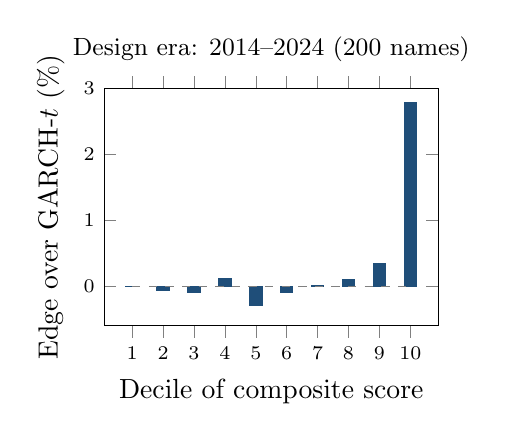
\begin{tikzpicture}
\begin{axis}[width=0.48\textwidth, height=4.6cm, ybar, bar width=4.5pt,
  xlabel={Decile of composite score}, ylabel={Edge over GARCH-$t$ (\%)},
  xtick={1,2,3,4,5,6,7,8,9,10}, ymin=-0.6, ymax=3.0,
  title={\small Design era: 2014--2024 (200 names)}, tick label style={font=\scriptsize}]
\addplot[fill=npblue, draw=npblue] coordinates
  {(1,-0.004)(2,-0.066)(3,-0.101)(4,0.119)(5,-0.287)(6,-0.089)(7,0.012)(8,0.108)(9,0.347)(10,2.787)};
\draw[gray,dashed,thin] (axis cs:1,0) -- (axis cs:10,0);
\end{axis}
\end{tikzpicture}\hfill
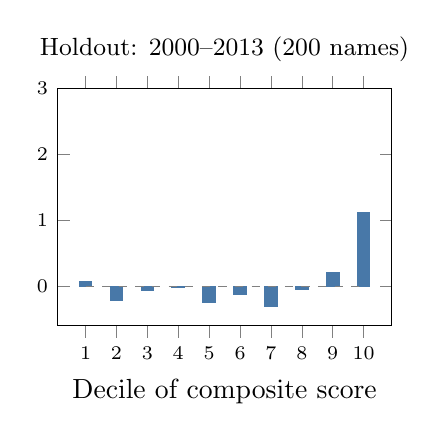
\begin{tikzpicture}
\begin{axis}[width=0.48\textwidth, height=4.6cm, ybar, bar width=4.5pt,
  xlabel={Decile of composite score},
  xtick={1,2,3,4,5,6,7,8,9,10}, ymin=-0.6, ymax=3.0,
  title={\small Holdout: 2000--2013 (200 names)}, tick label style={font=\scriptsize}]
\addplot[fill=npmid, draw=npmid] coordinates
  {(1,0.078)(2,-0.222)(3,-0.068)(4,-0.012)(5,-0.253)(6,-0.12)(7,-0.309)(8,-0.053)(9,0.207)(10,1.123)};
\draw[gray,dashed,thin] (axis cs:1,0) -- (axis cs:10,0);
\end{axis}
\end{tikzpicture}
\caption{The frontier in and out of era, by decile of the composite
misspecification score. Left: the design era (2014--2024). The top
decile carries $+2.79\%$ at per-date DM $8.9$, while deciles one through
nine sit within $\pm0.35\%$. Right: the composite score run
once on 2000--2013 CRSP data. The top decile carries $+1.12\%$ at
per-date DM $2.51$ over 1{,}465 dates. The threshold shape (edge
concentrated in the top decile, near zero elsewhere) reappears, as a
post-hoc check, in an era containing the 2008 crisis that no design stage used.}
\label{fig:holdout}
\end{figure}
The overall
signal--edge correlation is low (0.05--0.10) because the relationship
is a threshold nonlinearity, so the top-decile
Diebold--Mariano statistics are the appropriate summary.

\subsection{Beyond the equity panel}

Two kinds of evidence bear on other markets, and they differ in weight. The first is a study of the paper's estimator on fifteen instruments fixed, with its hypotheses, margins and tests, before their data were examined: six stocks outside the training pool, four exchange-traded funds on equities and credit, two on commodities, two currency pairs and ether, tested from 2020 to November 2026. Seventeen further instruments examined beforehand are reported as exploratory. The pooled parts of the estimator were trained once on the panel before 2020 and applied unchanged. Comparable is defined as a pooled FZ0 no more than 0.01 above the benchmark's, about the size of the estimator's gain over GARCH-$t$ on the panel. At 2.5\% the accuracy layer is comparable to GARCH-$t$, FHS, GARCH-EVT, EWMA and historical simulation on the fifteen, and to every benchmark, GJR-GARCH-skew-$t$ and Beta-$t$-EGARCH included, when all thirty-two are pooled and every model is fitted once before 2020. At 1\% the comparison is inconclusive: the estimator's point estimate is below GARCH-$t$'s, and the upper bounds on its excess loss against the GARCH family (0.014 to 0.018) exceed the margin. When the per-instrument benchmarks are refitted every year and the pooled parts are not, GJR-GARCH-skew-$t$ is ahead at 2.5\% on the fifteen (DM 2.06); most of that lead is the refit asymmetry and it falls within noise under a common protocol.

The post-shock mechanism is specific to stocks. On the days the score flags, Beta-$t$-EGARCH beats GARCH-$t$ by $4.8\%$ of 1\% pinball loss (DM 2.5) and $3.4\%$ at 2.5\% (DM 2.2) on the fourteen stocks, none of which is in the training pool, and it does not on the eighteen instruments in other asset classes ($-5.8\%$, DM $-1.6$, and $-2.0\%$, DM $-1.1$). The flexible tail on the robust scale gains $7.2\%$ and $5.0\%$ on the stocks' flagged days (DM 3.3 and 2.5); the accuracy layer on the GARCH-$t$ scale does not. We therefore claim the mechanism for individual stocks only. The protocol, the graded hypotheses and the deviations from it are in the Online Appendix.

The second kind of evidence is the set of exploratory sweeps of earlier versions: 24 currency pairs, 26 country indices, 43 cross-asset instruments and the Korea-2026 crash (Online Appendix Table~OA.20). They are not tests of the estimator. Each entry compares a standalone per-asset model with GARCH-$t$ on pinball loss; in the cross-asset sweep the entry is the better of FHS and the residual-hybrid on the test sample, FHS on 39 of the 43; and the currency entries come from the last of several specifications. We report them as description and draw no conclusion from their significance counts.

\subsection{Regime dependence and model selection}
\label{sec:gate}

In the amortized panel the absolute edge grows about fourfold with
turbulence, from 0.0059 in the calmest realized-vol quintile to 0.0247 in
the most turbulent, and both nonparametric estimators beat GARCH in every
quintile. Gating, running GARCH on calm days and the nonparametric model
when the score is high, does not improve on continuous use of the
flexible model: a classifier gate routes $90.5\%$ of days to the
nonparametric model and matches always-nonparametric exactly, and a
regression gate on the edge magnitude \citep{giacominiwhite2006} still
converges to it. This is consistent with Table~\ref{tab:frontier}: the
conditional mean of the loss differential is positive where the score is
high and indistinguishable from zero elsewhere, so no state pays to
select the parametric quantile, and the per-day oracle gap ($4.4\%$) is largely unforecastable from prior-day state. The amortized setting therefore uses the nonparametric
model throughout; the residual-hybrid is the choice where forecast accuracy no worse than GARCH-$t$ in the bulk is wanted, with the score as a monitor
(Section~\ref{sec:applications}).

%% ===== FRTB EVALUATION =====
\section{VaR and Expected Shortfall forecast evaluation}\label{sec:frtb}

\subsection{Head-to-head accuracy and significance}

Table~\ref{tab:frtb} reports the full comparison on the 200 CRSP names of Table~\ref{tab:frontier} (221.6k asset-days, 1{,}108 dates).

\begin{table}[t]
\centering
\begin{threeparttable}
\caption{FRTB comparison: average pinball loss (twelve quantile levels),
ES$_{97.5}$ calibration, and 99\% exception tests. 200 CRSP names, 221.6k
test asset-days.}
\label{tab:frtb}
\small\setlength{\tabcolsep}{4.5pt}
\begin{tabular}{lcccc}
\toprule
Model & Avg.\ pinball & ES$_{97.5}$ pred.\ vs realized & Breach$_{99}$ & Kupiec$_{99}$ $p$ \\
\midrule
\emph{Ideal value} & \emph{(smaller better)} & \emph{(pred.\ $=$ realized)} & \emph{1.00\%} & \emph{$>0.05$ (pass)} \\
\midrule
Residual-hybrid (GBM) & \textbf{0.3676} & $-6.64$ / $-6.12$ & 1.06\% & 0.01 \\
\quad $+$ EVT tail & 0.3680 & $-7.33$ / $-6.16$ & 0.87\% & 0.00 \\
GARCH(1,1)-$t$ & 0.3688 & $-6.98$ / $-5.92$ & 1.03\% & 0.167 \\
GJR-GARCH-skew-$t$ & 0.3688 & $-6.87$ / $-6.09$ & 1.02\% & 0.431 \\
GARCH-FHS (per-name) & 0.3689 & $-6.90$ / $-6.06$ & 1.08\% & 0.00 \\
GARCH-FHS (pooled) & 0.3691 & $-7.17$ / $-5.89$ & 0.97\% & 0.206 \\
GARCH-FHS (rolling 500d) & 0.3694 & $-7.02$ / $-6.21$ & 1.10\% & 0.00 \\
EWMA (RiskMetrics) & 0.3735 & $-5.72$ / $-5.84$ & 1.61\% & 0.00 \\
Historical simulation & 0.3752 & $-7.71$ / $-7.08$ & 0.87\% & 0.00 \\
\bottomrule
\end{tabular}
\begin{tablenotes}\footnotesize
\item All columns come from a single common-sample run, provided in
the replication package, on the 200 names and 1{,}108 test dates of
Table~\ref{tab:frontier} (221.6k asset-days), so the battery, the
frontier and the FZ0 comparison share one set of rows.
Predicted ES is the tail integral
$\alpha^{-1}\!\int_0^\alpha Q(v)\,dv$ of each model's quantile function: closed forms for the $t$ and
normal entrants, an exact substitution integral of the Hansen skew-$t$ inverse
CDF, the exact empirical tail mean for historical simulation and the FHS variants, and the converged integral of
Section~\ref{sec:hybrid} for the EVT-tailed residual-hybrid, whose VaR and ES are both read from
one monotonized min-envelope curve $Q^{z}_t$ of \eqref{eq:hybrid}. The raw residual-hybrid has no quantile below its lowest
fitted level, so its ES extends the body flat below $\alpha/40$ and is a lower bound on its severity.
Diebold--Mariano vs the residual-hybrid: GARCH-$t$ 6.2, GJR-skew-$t$ 5.6,
FHS pooled 6.9, per-name 6.3, rolling 6.0, HS 8.5, EWMA 9.6 (all
$p\approx0$, rounded, and stable across reruns). The EVT variant
concedes 0.0004 pinball (DM 7.0) to the first row, the raw
residual-hybrid without the tail, as the price of that tail. The 90\% MCS contains the
raw residual-hybrid alone, and CAViaR (separate common-sample run)
statistically ties it.
\item The ES columns are a diagnostic, not a ranking:
``realized'' is the mean return below each model's own VaR, so
the conditioning set is model-dependent, and under the numerical integral
each fat-tailed entrant exceeds its own-tail comparator by 8\% (raw
residual-hybrid, a lower bound) to 22\% (pooled FHS).
The joint Fissler--Ziegel score of the FZ0 re-scoring is the ranking
criterion for ES.
\item GJR-skew-$t$ row: Hansen inverse CDF with the fitted
degrees of freedom and skewness (median $4.2$ and $-0.015$), validated against the
symmetric-$t$ limit and against an independent reference implementation.
\item Exception columns are pooled panel diagnostics: at 221.6k
observations a breach-rate deviation of $\pm0.1$ points rejects in
either direction (the EVT variant's 0.87\% sits on the conservative
side; GARCH-$t$, GJR-skew-$t$ and pooled FHS land within 0.03 points of 1\%), so pooled $p$-values are
reported, not leaned on. The regulatory reading is the per-asset and
date-clustered restatement: per asset the EVT-tailed residual-hybrid of this
table passes Kupiec at 99\% for $86\%$ of names (Online Appendix Figure~OA.2), and the accuracy layer of the
FZ0 comparison passes Kupiec for $84\%$ and Christoffersen conditional coverage for $90\%$ (at 97.5\%, $70\%$ and $75\%$). On the date-clustered test it passes at 99\% ($t=0.62$) and is rejected marginally at 97.5\% ($t=2.00$), where GARCH-$t$ passes ($t=1.56$) and pooled FHS is rejected more strongly ($t=3.35$); its pooled body without the EVT tail is rejected at both levels ($t=4.3$ and $4.7$), so the tail stage carries the regulatory
calibration. All three pass on the 2000--2013 holdout, and the adaptive overlay of Stage~4 passes on both panels.
\end{tablenotes}
\end{threeparttable}
\end{table}

\paragraph{The stress-era replication.} The comparison set was re-run on the pre-committed 2000--2013 holdout panel. Splits follow
Section~\ref{sec:protocol}, so each name's test window runs from
roughly mid-2008 through 2013, the crisis and its aftermath. The
EVT-tailed residual-hybrid passes Kupiec at 99\% for $94\%$ of names and
Christoffersen for $95\%$, with date-clustered $t$-statistics of
$0.17$ at 99\% and $0.35$ at 97.5\%, consistent with nominal at both regulatory levels through the crisis window. Historical simulation and EWMA do not survive the same test: historical simulation
breaches at $1.53\%$ against a $1\%$ target (pass rate $61\%$,
date-clustered $t=2.08$) and EWMA at $1.57\%$ ($t=2.83$). GARCH-$t$ is also well calibrated in this era ($94\%$ pass rate), as the frontier predicts. Calibration parity is the norm, and the residual-hybrid's added value in any era is the accuracy edge where the misspecification score is high. The adaptive overlay of Stage~4 stays near nominal through the crisis window, breaching at $2.43\%$ and $2.38\%$ against the $2.5\%$ target and at $1.06\%$ and $1.04\%$ against $1\%$ for the two update rates (date-clustered $|t|\le0.44$).

\paragraph{Non-core comparisons.} Table~\ref{tab:noncore} adds two entrants from outside banks' standard toolkit. SAV-CAViaR, a leading semiparametric academic benchmark, ties the residual-hybrid, and the $90\%$ Model Confidence Set on that run contains exactly these two, so the residual-hybrid ties the strongest non-nested academic rival and significantly beats every model in banks' standard toolkit. The two tied models differ in what they deliver: SAV-CAViaR models one quantile level per fit, produces no ES (the FRTB metric) without an ad-hoc stage, and needs per-name history, so it cannot be applied to new listings; the residual-hybrid produces the full curve and extends to new listings. Pooled exception rejections are not counted against CAViaR, because pooled asset-day tests ignore cross-sectional dependence and overstate rejection for every model, the residual-hybrid included; the date-clustered restatement is the appropriate reading. A neural IQN used as the residual model loses to trees at both tunings (Table~\ref{tab:noncore}): the tail-aware, monotone, conformally recalibrated version narrows the untuned gap by an order of magnitude and repairs the thin tail, but the remaining deficit is still significant, so trees are the stronger tabular estimator and the residual-hybrid's edge does not rest on the choice of shape learner. Two textbook FHS variants, per-name train-constant and per-name rolling 500-day trailing, were run on the identical panel; both lose to the residual-hybrid (DM 5.2 and 5.7, pinball 0.3562 and 0.3569 against 0.3551) and bracket the pooled variant used in Table~\ref{tab:frtb}.

\begin{table}[htbp]
\centering
\begin{threeparttable}
\caption{Non-core comparisons. Each entrant is scored against the residual-hybrid on its own common sample, so loss levels are comparable within a row but not across rows.}
\label{tab:noncore}
\footnotesize\setlength{\tabcolsep}{5pt}
\begin{tabular}{lccccl}
\toprule
Entrant & Loss & Residual-hybrid & DM & Breach$_{99}$ & Verdict \\
\midrule
SAV-CAViaR & 0.3461 & 0.3460 & 0.4 & --- & tie ($p=0.34$) \\
Neural IQN, untuned & 0.3650 & 0.3551 & 13.3 & 3.2\% & loses \\
Neural IQN, tuned\tnote{a} & 0.3638 & 0.3632 & 3.03 & 0.92\% & loses \\
\bottomrule
\end{tabular}
\begin{tablenotes}[flushleft]\footnotesize
\item[a] Tail-aware $\tau$-sampling, monotone rearrangement, and a per-level conformal shift calibrated on the first half of the test window and scored on the second half; the residual-hybrid in this row is recalibrated the same way, so the loss levels are not comparable with Table~\ref{tab:frtb}.
\item DM is the per-date Diebold--Mariano $t$-statistic against the residual-hybrid; positive favors the residual-hybrid. The $90\%$ Model Confidence Set contains the residual-hybrid alone on the Table~\ref{tab:frtb} run, and the residual-hybrid together with CAViaR on the CAViaR run. Breach rates were not computed for the CAViaR run, which reports one quantile level per fit.
\end{tablenotes}
\end{threeparttable}
\end{table}


\paragraph{The joint $(\VaR,\ES)$ score.} Because ES is not elicitable
alone but the pair $(\VaR,\ES)$ is jointly elicitable under the
Fissler--Ziegel class \citep{fissler2016}, the comparison set was also scored under the FZ0 joint score
\begin{equation}
L_{\mathrm{FZ0},\alpha}(r,q,e)=-\frac{1}{\alpha e}\,\mathbb{I}\{r\le q\}(q-r)
+\frac{q}{e}+\log(-e)-1,\qquad e\le q<0,
\label{eq:fz0}
\end{equation}
the $0$-homogeneous member of the class \citep{patton2019}. Lower values are better. 

\begin{figure}[t]
\centering
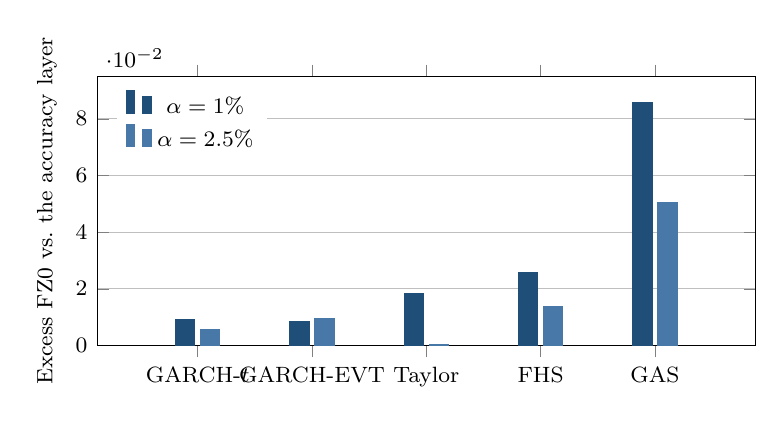
\begin{tikzpicture}
\begin{axis}[width=0.82\linewidth,height=5cm, ybar, bar width=7pt,
  ymin=0, ymax=0.095, ylabel={Excess FZ0 vs.\ the accuracy layer},
  symbolic x coords={GARCH-$t$,GARCH-EVT,Taylor,FHS,GAS}, xtick=data,
  enlarge x limits=0.22, ymajorgrids,
  legend style={font=\footnotesize,at={(0.03,0.97)},anchor=north west,draw=none},
  tick label style={font=\footnotesize}, label style={font=\footnotesize}]
\addplot[fill=npblue,draw=npblue] coordinates {(GARCH-$t$,0.00919)(GARCH-EVT,0.00861)(Taylor,0.01819)(FHS,0.02588)(GAS,0.08585)};
\addplot[fill=npmid,draw=npmid] coordinates {(GARCH-$t$,0.00557)(GARCH-EVT,0.00963)(Taylor,0.00036)(FHS,0.01382)(GAS,0.05042)};
\legend{$\alpha=1\%$,$\alpha=2.5\%$}
\end{axis}
\end{tikzpicture}
\caption{Joint (VaR, ES) FZ0 loss of each benchmark in excess of the
residual-hybrid's accuracy layer (the EVT-tailed variant without the
conformal shift), on the full 200-name panel. A positive bar
means worse than the accuracy layer. Among the industry-standard benchmarks the accuracy layer (the zero baseline) has the
lowest FZ0 at $1\%$ and is never significantly beaten at $2.5\%$, beating GARCH-$t$ (DM $4.9$ at
$1\%$, $5.5$ at $2.5\%$), pooled-tail GARCH-EVT (DM $4.5$ and $6.3$) and per-name FHS (DM $4.9$ and $5.4$), together with the two
FZ-estimated dynamic-ES benchmarks fitted per name by multi-start FZ0
minimization, the generalized autoregressive score (GAS) model of \citet{patton2019} (DM $9.9$ and $8.8$) and the
ES-CAViaR of \citet{taylor2019} (DM $3.8$ at $1\%$, a tie at $2.5\%$). Every bar and DM comes from one run on the same rows against the same accuracy-layer forecast. SAV-CAViaR, scored on its own common sample (Table~\ref{tab:noncore}), ties the accuracy layer and is omitted here; the adaptive overlay, within noise of the accuracy layer at both levels, is discussed in the text. A Beta-$t$-EGARCH, outside the industry-standard set, scores below the accuracy layer at both levels under these frozen fits (DM 2.48 at $2.5\%$) and is within noise of it under annual refits (text).}
\label{fig:fz0}
\end{figure}

On the full 200-name panel ($221.6$k test asset-days), VaR and ES are read from the coherent min-envelope curve $Q^{z}_t$ of \eqref{eq:hybrid} and per-date DM inference is used throughout. The residual-hybrid's \emph{accuracy layer}, the EVT-tailed variant with no conformal shift, attains the lowest FZ0 of the industry-standard benchmarks of Section~\ref{sec:background} (historical simulation, EWMA, GARCH-$t$, GJR-GARCH-skew-$t$ and FHS) at 1\% and is never significantly beaten by them at 2.5\%. At 1\% it beats GARCH-$t$ (DM 4.9) and FHS (DM 4.9), the two standard benchmarks the accuracy claim rests on. At 2.5\% it again wins over GARCH-$t$ (DM 5.5). On the same rows it also beats standalone GARCH-EVT, whose ES is the McNeil--Frey closed form, with a pooled tail by DM 4.5 at 1\% and 6.3 at 2.5\%, and per name by DM 5.1 and 5.4, so the gain over the conventional EVT construction is not confined to the pinball frontier. The dynamic quantile test of \citet{engle2004caviar} (four hit lags and the VaR) passes at the 5\% level for 86\% of names at 1\% and 70\% at 2.5\% for the accuracy layer, against 84\% and 68\% for GARCH-$t$ and 83\% and 62\% for the pooled GARCH-EVT. Because a ranking under one consistent score need not hold under another \citep{patton2020}, the Online Appendix reports Murphy diagrams \citep{ehm2016} for the VaR forecasts: the accuracy layer has the lower elementary score against GARCH-$t$ on 70\% of the threshold grid at 1\% and 65\% at 2.5\%, and against the pooled GARCH-EVT on 85\% at both levels, losing in a band of thresholds near the typical VaR level. Extending the joint score to the whole comparison set on the same rows (Online Appendix Table~OA.11), the accuracy layer has the lowest mean FZ0 of the benchmark models at 1\%, a level statement since GJR-GARCH-skew-$t$ is within noise (DM 1.2). At 2.5\% the accuracy layer, GJR-GARCH-skew-$t$ and the Taylor model form a tie group (FZ0 1.8486, 1.8486 and 1.8490; DM $-0.02$ and 0.1), and nothing significantly beats the accuracy layer; its own pooled body, without the EVT branch, scores lower still (DM $-1.1$ at 1\% and $-1.5$ at 2.5\%, both within noise) while breaching at 1.3\% and 3.3\%, the coverage cost the EVT branch removes; the 90\% Model Confidence Set on the per-date FZ0 series contains the accuracy layer, the pooled body and GJR-GARCH-skew-$t$ at 1\% (with the static-shift row, identical to the accuracy layer at that level) and the accuracy layer, the pooled body, GJR-GARCH-skew-$t$ and the Taylor model at 2.5\%, and excludes GARCH-$t$, every FHS variant, both GARCH-EVT forms, the GAS model, EWMA and historical simulation at both levels. On the eleven-level pinball the set contains the pooled body and SAV-CAViaR and excludes the accuracy layer, since the EVT branch costs pinball, as Table~\ref{tab:frtb} reports for the twelve-level battery, and is kept for the exception tests it passes. The two closest dynamic $(\VaR,\ES)$ benchmarks are the one-factor score-driven GAS of \citet{patton2019} and the ES-CAViaR of \citet{taylor2019}. Each is estimated per name by minimizing the same FZ0 loss on the last 1{,}200 days of the estimation window, from three starts. The GAS scales are fixed at that window's empirical VaR and ES, so it is a restricted form of the model; it scores below GARCH-$t$ and is a weak benchmark. Refitted on the whole estimation window with a longer optimiser, the Taylor model converges for all $200$ names and the comparison is unchanged (DM 3.2 at 1\%, a tie at 2.5\%), though in the top decile of the score it is ahead of the accuracy layer (DM $-1.8$ and $-2.6$); with its scales estimated the GAS improves at 1\% without closing the gap (DM 10.8) and is unstable out of sample at 2.5\% (Online Appendix). The accuracy layer beats the GAS at both levels (DM 9.9 at 1\%, 8.8 at 2.5\%), and it beats the Taylor model at 1\% (DM 3.8) while tying it at 2.5\%, the near-tie the fat-tailed benchmarks all show at 2.5\% where the shape edge is thin. A score-driven Beta-$t$-EGARCH \citep{harvey2013dynamic}, outside the industry-standard set, has lower FZ0 at both levels under the frozen fits, significantly at 2.5\% (DM 2.48). Under the annual refits of Section~\ref{sec:calendarleak} the two are within noise overall, with the accuracy layer slightly ahead (DM 1.2 and 0.9), while Beta-$t$-EGARCH stays significantly ahead in the top decile of the score (DM 3.7 and 5.1). Its bounded response to a shock removes the post-shock variance overstatement of Section~\ref{sec:frontier}, the frontier's own mechanism, and refitting does not.

This ranking survives the annual walk-forward refit of Section~\ref{sec:calendarleak}: re-estimating every stage at each January-1 cutoff and re-scoring the 2020--2024 panel, the accuracy layer keeps a lower FZ0 than both refitted benchmarks at both levels, beating GARCH-$t$ by DM 3.5 at 1\% and 3.1 at 2.5\%, and pooled FHS, the unconditional residual quantile on the same refitted scale, by DM 3.2 and 3.4 (one-sided $p<0.005$). Refitting narrows these margins without closing them, unlike the average pinball edge, which closes under the same refit. With Beta-$t$-EGARCH in place of GARCH-$t$ as Stage 1, the engine has lower FZ0 under the frozen fits (DM 3.16 and 4.37, and 3.14 and 3.63 on the 2000--2013 holdout). Under annual refits the two engines are within noise overall (DM $-0.31$ and $-0.02$), and the Beta-$t$-EGARCH engine is ahead in the top decile of the score (DM 5.46 and 7.37), so refitting does on average what a robust filter does but leaves the post-shock error in the states the score flags. Stage 1 stays GARCH-$t$ under the rule fixed before the refit run.

The accuracy layer is thus one configuration that is never significantly beaten on FZ0 by the industry-standard benchmarks at either level, scores lowest at 1\%, and passes the aggregate date-clustered exception test at 99\%. At 97.5\% it is rejected marginally on 2020--2024 ($t=2.00$, against 1.56 for GARCH-$t$ and 3.35 for pooled FHS) and passes on the 2000--2013 holdout ($t=0.25$), a test with little power there: its clustered standard error for the accuracy layer is 0.53 points at $1\%$ and 0.28 at $2.5\%$, so it rejects no breach rate below $2.05\%$ at $1\%$ or inside $1.95$--$3.05\%$ at $2.5\%$. Per-name diagnostics show residual cross-sectional calibration heterogeneity (84\% and 90\% pass rates at 99\%). The pooled 221.6k-observation Kupiec test also rejects at 97.5\%, and at this sample size it rejects very small deviations. The joint-score edge over GARCH-$t$ is less concentrated than the pinball edge: at 1\% the mean FZ0 gap is 0.011 in the top misspecification decile and 0.009 in the other nine (DM 3.4 and 4.7). That flatness is a property of the splice. The pooled GPD is unconditional, so in the top decile it overrides a body that has pulled its tail in; the unconditional tail buys about 0.3 points of 97.5\% coverage at a cost of 0.06 to 0.07 in top-decile FZ0, and the paper keeps it for the coverage (Online Appendix).

\paragraph{The adaptive overlay.} Stage~4 shifts the accuracy layer by a scalar updated each day from the panel breach frequency (Section~\ref{sec:hybrid}). Before the run we fixed the rule under which it would be switched on: on both the 2014--2024 panel and the 2000--2013 holdout, at both update rates, the overlay had to bring the 97.5\% breach rate within 0.3 points of nominal and keep its FZ0 within noise of the accuracy layer ($|\mathrm{DM}|<2$) at both levels. It meets both conditions. In era it moves the 97.5\% breach rate from 2.78\% to 2.68\% and 2.60\% for $\gamma=0.02$ and $0.05$, with FZ0 slightly below the accuracy layer's (DM $-1.3$ and $-1.0$), and the date-clustered test passes ($t=1.30$ and $0.78$); at 99\% it leaves the accuracy layer essentially unchanged (DM $-0.3$ for both rates). On the holdout its breach rates are 2.43\% and 2.38\% at 97.5\% and 1.06\% and 1.04\% at 99\%, with every $|\mathrm{DM}|$ against the accuracy layer below 1. It keeps the joint-score lead over GARCH-$t$ at 2.5\% in era (DM 5.2 and 4.1). In the top misspecification decile it concedes 2.5\% FZ0 to the accuracy layer (DM 3.4 and 3.6), the price of widening the band where it is already widest. A static shift, the construction of earlier versions, fails in both of its forms. Estimated on the body's calibration errors and applied to the envelope, it counts the tail correction twice and over-covers (breach 1.66\%, date-clustered $t=-9.1$, FZ0 DM 2.6 against the accuracy layer); estimated on the envelope's own errors, it still over-covers in era (2.15\%, $t=-3.1$), because the calibration block and the test era miss on opposite sides of nominal. Each ``lowest FZ0'' statement refers to the accuracy layer.

\paragraph{Direct ES calibration backtests.} Because exception counts test VaR and not ES, the exceedance-residual test of \citet{mcneilfrey2000} and the $Z_2$ statistic of \citet{acerbi2014backtesting} complement the FZ0 comparison \citep{noldeziegel2017elicitability, bayer2022esr}. Neither rejects the residual-hybrid's ES on the design panel or under annual refits, while GARCH-$t$'s 1\% ES is rejected as not severe enough. On the 2000--2013 holdout the 1\% test rejects every construction, in opposite directions: GARCH-$t$'s ES as not severe enough and the residual-hybrid's and FHS's as too severe. The full results are in the Online Appendix (Table~OA.5).

\paragraph{The ten-day horizon.} A separate direct model trained on ten-day returns beats $\sqrt{h}$-scaled GARCH by about 1.4\% of pinball on 2014--2024, and about half of that edge is the scaling rule itself. On the pre-committed 2000--2013 rerun it ties the iterated GARCH benchmarks and the scaled parametric tail is the better calibrated. The ten-day evidence is mixed; it is reported in the Online Appendix (Table~OA.13), and no ten-day claim attaches to the one-day estimator.

\subsection{Cross-asset evidence}

Across the 43-instrument sweep the relationship is heterogeneous. The volatility indices (VIX, V2X, VVIX) and Baltic freight post the largest accuracy gains and survive the multiplicity adjustment (Online Appendix Table~OA.4), but their calibration is open. VIX's breach-independence is marginal (one-sided $p=0.041$), and credit and Baltic freight fail it, so all are reported as accuracy edges and none as a calibrated win. Instrument-level results and diagnostics are
collected in the Online Appendix.

\paragraph{The scale--shape decomposition.} Against a Realized GARCH \citep{hansen2012realized} fitted on intraday data, the daily-data core concedes FZ0 at both levels (DM $6.2$ and $4.6$). Re-fitting the shape learner, EVT tail, and score on the realized residuals, however, leaves the score's edge within noise. On large caps the frontier is therefore largely daily-scale misspecification. Where intraday data are unavailable or too sparse to build a realized measure (new listings, illiquid names, many cross-asset instruments), the daily score is the version of the diagnostic that can be computed (Online Appendix).

%% ===== APPLICATIONS =====
\section{Extensions and implications}\label{sec:applications}



\paragraph{Using the score.} The score is available \emph{ex ante}: a
risk manager computes today's value from today's residuals and uses it
for tomorrow's forecast. Its role is to stratify, not to switch models
day by day, because the per-day oracle gap ($4.4\%$) is largely unforecastable from
prior-day state and a learned gate collapses to always-nonparametric
(Section~\ref{sec:gate}). It drives a switch in two settings: the per-name
standalone model, where nonparametric quantiles underperform
on calm days, and the choice of Stage-1 scale, described next. As a monitor it is cheap, since its input is the trailing
residual window the scale stage already produces, and it is a slow state
that need not be watched daily. On capital, the residual-hybrid is a
one-day single-name VaR/ES forecaster of the kind that feeds an internal
model, not the ten-day portfolio-level stressed ES that sets the FRTB
charge; the paper makes no capital-release claim, because the
predicted-versus-realized ES wedge conditions on each model's own breach
set and no defensible arithmetic converts it to capital
\citep{bcbs2019frtb}. The narrower implication is that the ES-based
component of the charge scales with the ES forecast.

\paragraph{Choosing the scale with the score.} Under the annual refits the Beta-$t$-EGARCH engine and the GARCH-$t$ engine are within noise overall while the robust one leads in the top decile of the score (Section~\ref{sec:frtb}), which suggests letting the score choose the scale. A gate that runs the GARCH-$t$ engine when the previous day's $\mathrm{mk}_{63}$ is below its pre-2020 90th percentile, a threshold fixed before the first test year, and the Beta-$t$-EGARCH engine otherwise switches on 10.0\% of the 251.6k refit test asset-days. Its joint score is significantly better than always running the GARCH-$t$ engine (DM 6.3 at 1\%, 8.1 at 2.5\%) and statistically equal to always running the Beta-$t$-EGARCH engine (DM 0.8 at both levels), which is slightly ahead of it in the top decile (DM $-1.6$ and $-1.7$, within noise); the gate and both fixed engines pass the date-clustered exception test at both levels. The gate keeps the paper's Stage-1 filter on nine asset-days in ten and recovers the robust scale's gain where the score is high. Where tail accuracy is the only objective, running the robust scale everywhere does as well. The gate was designed after the robust filter's top-decile lead had been seen on these rows, so this is a description of the panel and not an out-of-sample test. On thirty-two instruments outside the panel, with every model fitted before 2020, the same rule does not beat GARCH-$t$ (DM $-1.1$ at 1\% and $-0.4$ at 2.5\%), and on the fourteen stocks among them its gain on flagged days is positive and not significant (Online Appendix).

\paragraph{New listings.} Because the shape model is pooled across names, a variant that conditions on characteristics alone can be evaluated for an asset with no return history. So can a simple pooled peer proxy, the median EWMA scale of other recent listings times pooled empirical residual quantiles, and that is the comparator a risk desk would reach for. On 303 names listed from 2018, scored out of time against that proxy on the same rows, the characteristics-only form built without look-ahead loses in every age bucket from the first week to six months (its mean pinball is 1.2 to 2.5\% higher), and in the first five trading days the proxy itself breaches its 1\% VaR on 7.1\% of asset-days. Day-one forecasts from characteristics are therefore available, not more accurate. Once a name has a few days of returns the full amortized model, whose inputs are mostly the name's own recent returns, beats the peer proxy by 5.5\% of pinball at ages two to five days (DM 4.9) and by 11 to 14\% from the second week through the first year (DM 7.3 to 20.1), and it beats the expanding-window Gaussian own-history benchmark by 7.6\% at 15 to 60 days (DM 6.8). Pooled own-history rivals also beat the peer proxy by 10 to 13\%, so the amortized model's margin over the strongest own-history alternative is probably small, and the paper treats transfer to new names as a secondary result. The ablation of Section~\ref{sec:gbcmethod} traces the handover from characteristics to the name's own volatility as its history lengthens.

% Trading implications and scenario generation are discussed in the Online Appendix.

\section{Conclusion}\label{sec:limitations}

Flexible tail-risk models beat GARCH(1,1)-$t$ on a narrow set of asset-days, about one in ten, and a trailing kurtosis of the filter's own residuals identifies them a day ahead; the next tenth carries a smaller edge and elsewhere they do not measurably improve on it. A high score is mostly a record of one recent large shock and of the variance the filter carries after it, and most of what flexible models earn on those days is a correction to that variance: a filter that bounds the shock's influence earns as much with a Student-$t$ tail and beats both flexible models studied there. A smaller residual-shape component survives on a robust scale and lowers the joint $(\VaR,\ES)$ loss at both regulatory levels. The semiparametric estimator used to measure all of this ties the best parametric benchmarks on the joint score rather than beating them; its value is diagnostic, in showing where and why the standard filter is stressed. The evidence is for individual stocks: on other asset classes the estimator is comparable to the standard benchmarks at 2.5\% and the post-shock mechanism does not appear. Transfer to newly listed names is a secondary result: once a name has a few days of returns the pooled model beats a peer proxy, but its characteristics-only day-one form does not (Section~\ref{sec:applications}).

These conclusions carry qualifications. The score is predictive rather than a necessary or sufficient condition: high residual kurtosis coincides with ties in some markets, and in credit and freight the accuracy edges sit alongside failed breach-independence tests. The accuracy layer's 97.5\% coverage is rejected marginally on 2020--2024 (date-clustered $t=2.00$, against 1.56 for GARCH-$t$), which the adaptive overlay repairs at no cost in FZ0. The McNeil--Frey exceedance-residual test rejects none of the residual-hybrid's ES forecasts on the design panel or under annual refits, but on the 2000--2013 holdout it rejects the 1\% ES of every construction tried, the residual-hybrid's and FHS's as too severe and GARCH-$t$'s as not severe enough. The shape component is the smaller part of the edge, since the decomposition attributes most of it to daily-scale misspecification that a jump-robust or realized-variance scale removes (Sections~\ref{sec:frontier} and \ref{sec:frtb}), and what survives is real but modest; on a robust scale it sits in the tail, where the flexible tail still lowers the joint $(\VaR,\ES)$ loss at both regulatory levels under frozen fits and annual refits. Where intraday data are too sparse to build a realized measure, the daily model and its score remain the available tool. The ten-day extension is a separate direct model whose in-era edge does not survive the 2000--2013 rerun (Online Appendix). And the score serves as a monitor rather than a day-to-day switch between parametric and flexible shapes, since the day-ahead oracle gap is largely unforecastable (Section~\ref{sec:gate}). On the panel a gate that moves to Beta-$t$-EGARCH in the score's top decile is significantly better than GARCH-$t$ at both levels; it was designed on those rows and does not beat GARCH-$t$ on instruments outside the panel (Section~\ref{sec:applications}).
Distributional uncertainty around these VaR and ES forecasts and the multivariate portfolio tail are left to future work.

\section*{Funding}
This work was supported by the Northwestern University Department of
Statistics and Data Science [Undergraduate Research Fellowship Grant,
2026].

\section*{Acknowledgments}
I thank Wenxin Jiang for his advice and guidance throughout this
research, and seminar participants and colleagues for comments. All
errors are mine.
AI assistance (Anthropic's Claude) was used in drafting, editing, and
code development; the author designed the research, verified all
results, and is responsible for the content.

\section*{Conflict of interest}
The author declares no conflicts of interest.

\section*{Ethics statement}
This study uses licensed secondary market data (CRSP/WRDS and
Bloomberg) under the terms described in the data availability
statement. It involves no human subjects and required no ethics
approval.

\section*{Data and code availability}
\addcontentsline{toc}{section}{Data and code availability}
A public replication package at
\href{https://github.com/sean-qin-usa/downside-risk-paper}{\texttt{github.com/sean-qin-usa/downside-risk-paper}}
covers every WRDS-based table and figure in this paper and preserves
the Bloomberg-based exhibits as run from their derived series. It
provides estimation code for all stages of the estimator
(\eqref{eq:garch}--\eqref{eq:hybrid}), the misspecification score
\eqref{eq:score}, the FRTB comparison, and the walk-forward schedule, seeds, and hyperparameter grids
referenced in the text, together with a mapping from each table and
figure to the script and result file that produce it. Return data
derive from CRSP, Bloomberg, and OptionMetrics under the author's
institutional licenses and cannot be redistributed; the package
includes the code to rebuild each panel from those sources, the derived
non-proprietary series, and a synthetic example dataset on which the
full pipeline runs end-to-end without licensed data. The holdout's
frozen specification, including its written-in-advance predictions, is
recorded in the package alongside the design-era pipeline so that the
two can be compared line by line. A citable archival snapshot (Zenodo
DOI) will be minted for the accepted version.


%% ===== BIBLIOGRAPHY =====
\bibliographystyle{apalike}
\bibliography{refs_v3}

% Proofs and supplementary exhibits are in the Online Appendix.

\end{document}
